%! TeX root = ../main.tex
\chapter{THIẾT KẾ HỆ THỐNG NUTRICARE}

Chương này trình bày thiết kế kỹ thuật và cách vận hành thực tế của ứng dụng NutriCare dựa trên các cơ sở lý thuyết đã xây dựng ở Chương 2. Nội dung tập trung vào bốn phần trọng tâm: câu chuyện người dùng và phân quyền sử dụng, kiến trúc tổng thể hệ thống, thiết kế cơ sở dữ liệu, các luồng xử lý chính và giao diện ứng dụng di động.

\section{Câu chuyện người dùng và phạm vi phân quyền}
\label{sec:user-stories}

Để người dùng có thể tra cứu nhanh ngay tại siêu thị mà vẫn đáp ứng nhu cầu quản lý dinh dưỡng dài hạn cho người bệnh, ứng dụng hỗ trợ hai chế độ sử dụng ngay từ lúc mở app: \textbf{chế độ Khách (không cần đăng nhập)} và \textbf{chế độ Đã đăng nhập Google}. Thanh điều hướng chính luôn giữ cố định bốn mục gồm \textit{Tra cứu}, \textit{Tiến trình}, \textit{Lịch sử} và \textit{Hồ sơ}. Ở chế độ Khách, người dùng vẫn quét ảnh và xem lại lịch sử bình thường, còn hai mục \textit{Tiến trình}, \textit{Hồ sơ} cùng chức năng tư vấn AI sẽ hiển thị biểu tượng ổ khóa kèm nút mời đăng nhập ngay tại chỗ. Bảng~\ref{tab:user-stories} tóm tắt các nhu cầu sử dụng chính của hệ thống.

\begin{table}[htbp]
    \centering
    \caption{Các câu chuyện người dùng (User Story) và phạm vi sử dụng của NutriCare}
    \label{tab:user-stories}
    \begingroup
    \small
    \setlength{\tabcolsep}{5pt}
    \renewcommand{\arraystretch}{1.22}
    \begin{tabularx}{\textwidth}{@{}>{\bfseries\raggedright\arraybackslash}p{1.3cm}>{\raggedright\arraybackslash}p{2.9cm}X@{}}
        \toprule
        Mã & Vai trò sử dụng & Nhu cầu của người dùng \\
        \midrule
        US1 & Khách chưa đăng nhập & Mở ứng dụng chụp hoặc chọn ảnh thực phẩm để nhận diện nguyên liệu, đọc khối lượng trên tem nhãn, chọn phần thịt hoặc loại trứng, điều chỉnh tỷ lệ ăn thực tế $\gamma$ và xem lại danh sách đã tra cứu trên điện thoại mà không bị bắt buộc đăng nhập. \\
        US2 & Người dùng Google & Đăng nhập tài khoản Google để mở khóa phần hồ sơ cá nhân, tải lại lịch sử cũ từ đám mây và tự động gộp những món đã quét khi còn ở chế độ Khách vào tài khoản cá nhân. \\
        US3 & Người dùng theo dõi sức khỏe & Nhập các chỉ số cơ thể, dị ứng và 6 bệnh lý mạn tính (kèm tùy chọn chế độ kiểm soát béo phì khi $\mathrm{BMI} \ge 23{,}0$), chủ động chọn món đưa vào thực đơn ngày để xem tiến độ calo, vi chất và cảnh báo vượt ngưỡng an toàn. \\
        US4 & Người dùng cần tư vấn chuyên sâu & Yêu cầu trợ lý AI đánh giá khẩu phần thực ăn hiện tại $m_{\text{consumed}}$ có phù hợp với tình trạng bệnh lý của mình hay không và gợi ý thêm nguyên liệu tươi sống bổ sung an toàn. \\
        \bottomrule
    \end{tabularx}
    \endgroup
\end{table}

\section{Kiến trúc tổng thể hệ thống}
\label{sec:system-architecture}

NutriCare được thiết kế theo mô hình kết hợp giữa \textbf{xử lý trực tiếp trên điện thoại} và \textbf{dịch vụ máy chủ đám mây} (Hình~\ref{fig:system_architecture}). Cách tổ chức này giúp các tác vụ quét ảnh, đọc nhãn cân và tra cứu bảng dinh dưỡng chạy hoàn toàn ngoại tuyến với tốc độ phản hồi nhanh, trong khi các tác vụ cần bảo mật khóa API, lưu trữ dài hạn và gọi mô hình ngôn ngữ lớn được đặt tập trung ở máy chủ.

\begin{figure}[htbp]
    \centering
    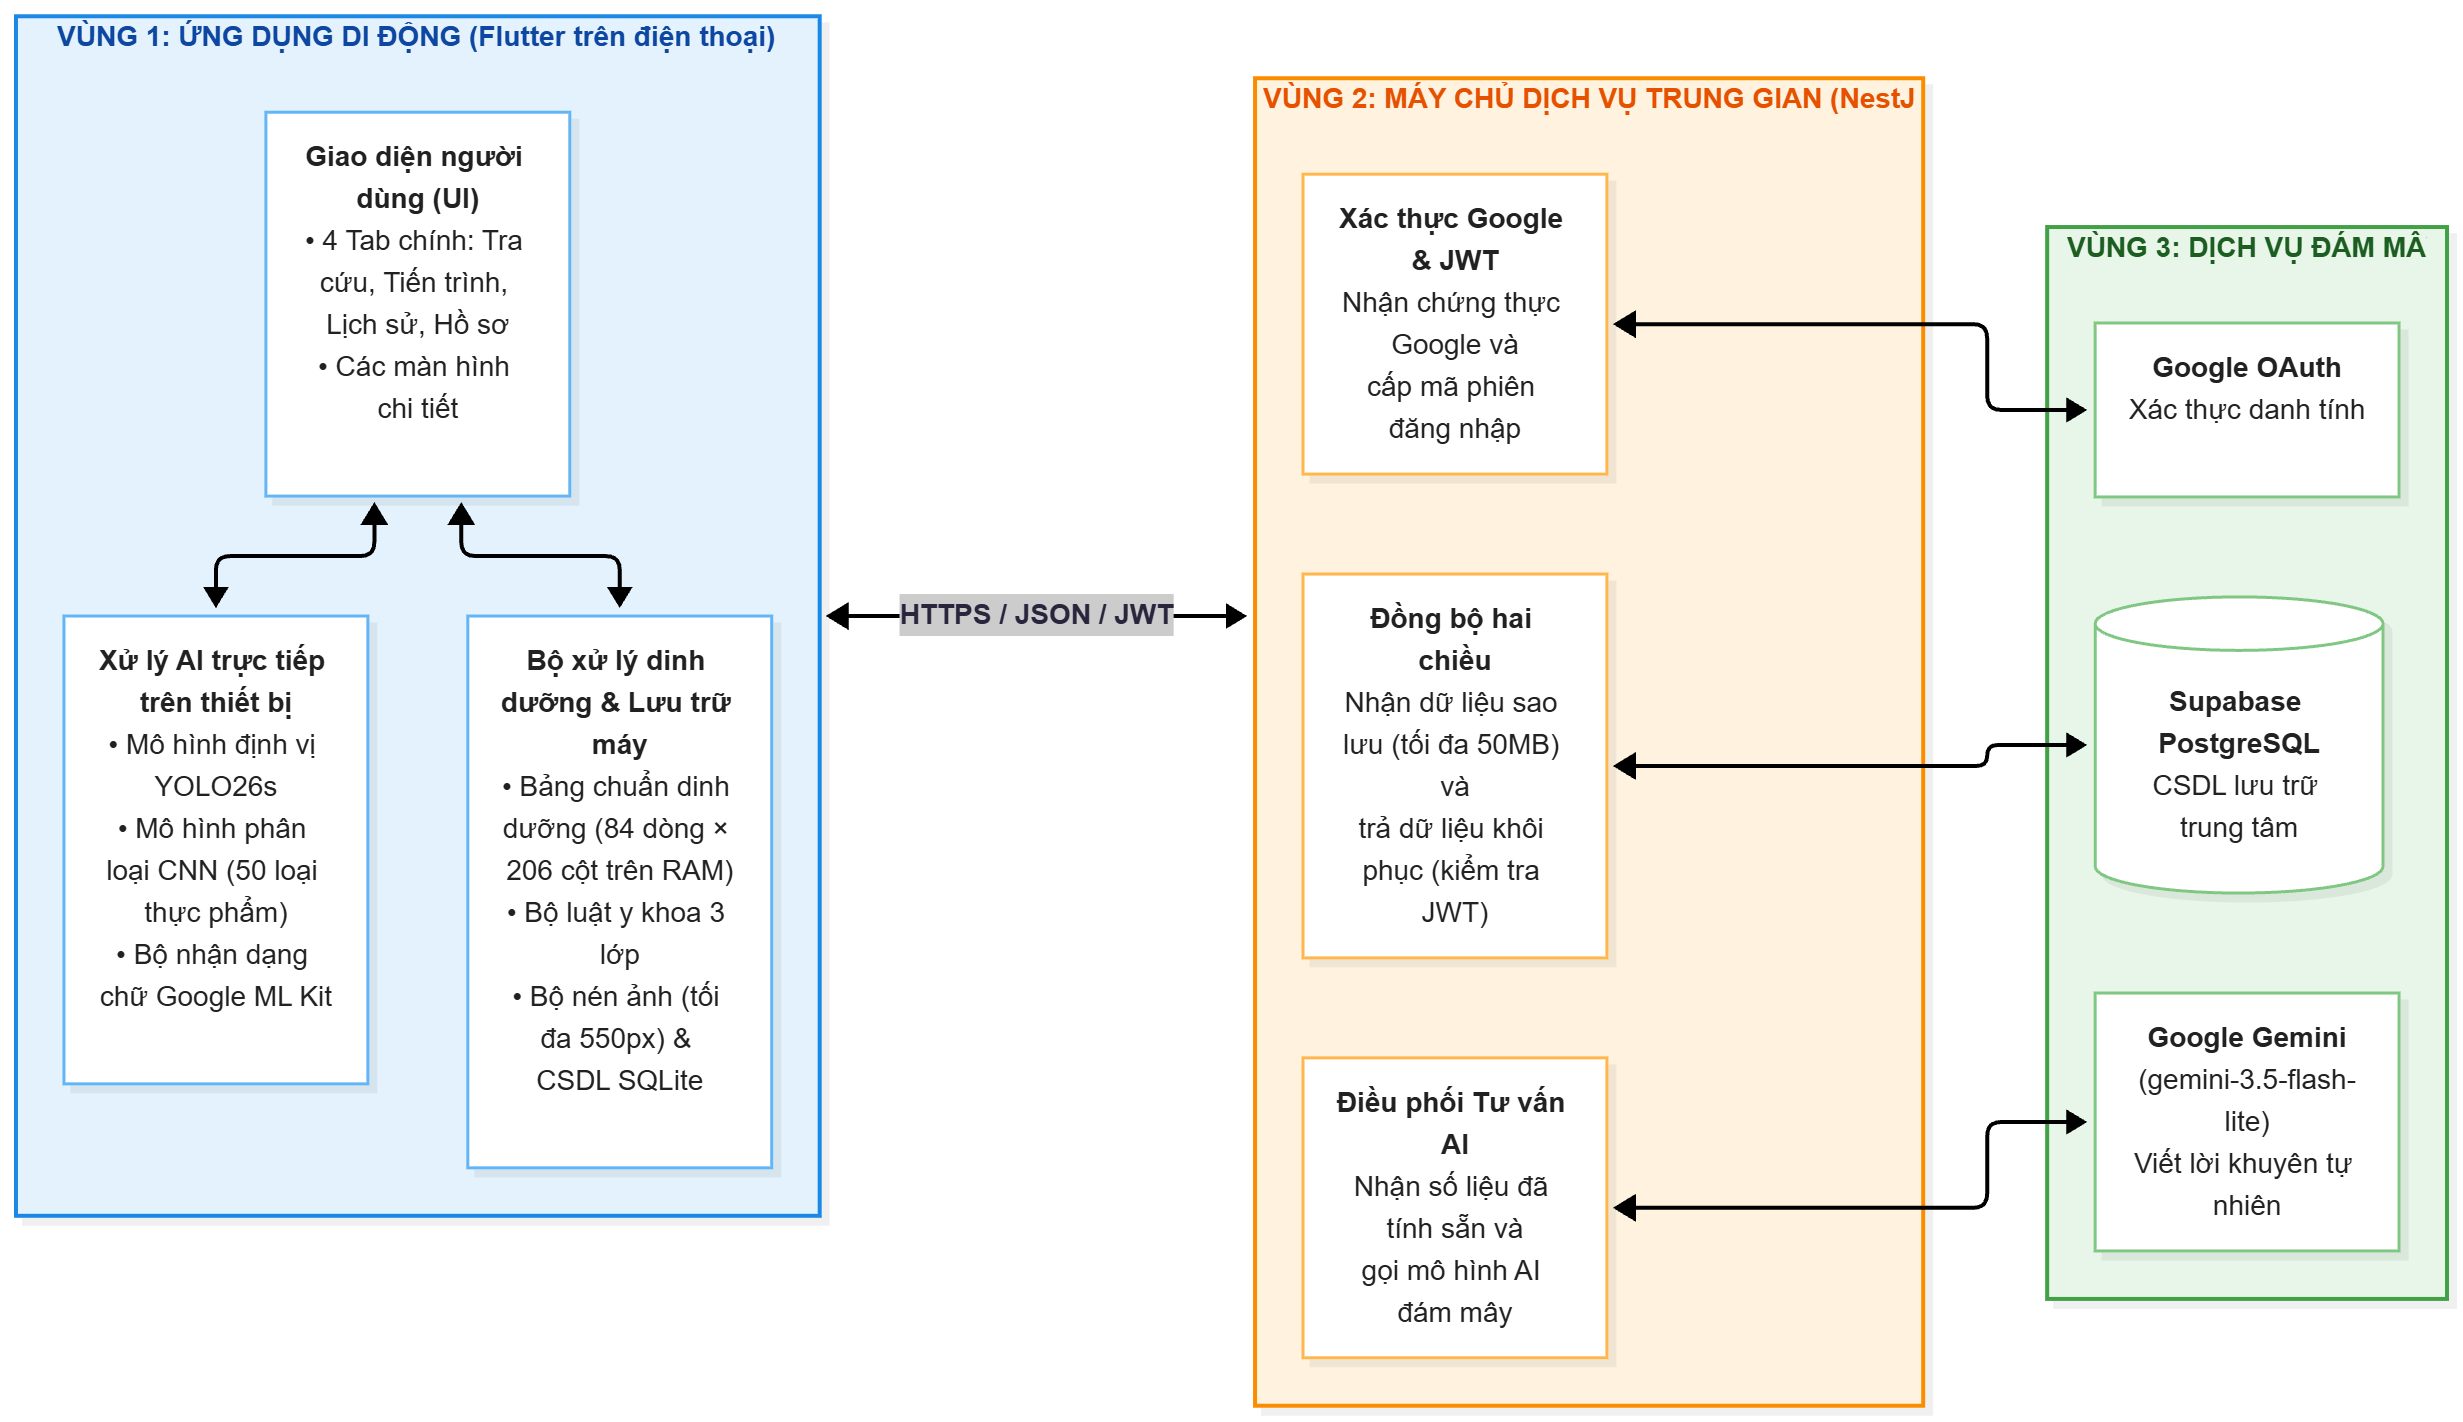
\includegraphics[width=0.95\textwidth,height=0.45\textheight,keepaspectratio]{so_do_kien_truc_he_thong.png}
    \caption{Kiến trúc tổng thể hệ thống NutriCare kết hợp xử lý trên thiết bị và dịch vụ đám mây}
    \label{fig:system_architecture}
\end{figure}

Hệ thống chia thành bốn lớp thành phần chính trao đổi dữ liệu qua giao thức HTTPS bảo mật:
\begin{enumerate}[leftmargin=0.8cm, itemsep=3pt, topsep=2pt]
    \item \textbf{Ứng dụng di động (Flutter):} Thực thi các mô hình trí tuệ nhân tạo biên (YOLO26s định vị vùng ảnh, mạng nơ-ron tích chập phân loại 50 nguyên liệu và thư viện nhận dạng chữ Google ML Kit) trên luồng xử lý nền để giao diện luôn mượt mà; nạp sẵn bảng thành phần dinh dưỡng vào bộ nhớ; chạy bộ kiểm tra an toàn y khoa tại máy; nén ảnh tối đa $550\text{ px}$ và lưu dữ liệu bằng SQLite.
    \item \textbf{Máy chủ dịch vụ trung gian (NestJS):} Đóng vai trò cổng điều phối gồm ba phân hệ: xác thực tài khoản Google và cấp mã phiên đăng nhập JWT; đồng bộ hai chiều dữ liệu sao lưu/khôi phục có kiểm tra quyền truy cập và hỗ trợ gói dữ liệu ảnh nén tới $50\text{ MB}$; và chuẩn hóa yêu cầu tư vấn dinh dưỡng trước khi chuyển lên mô hình ngôn ngữ lớn.
    \item \textbf{Dịch vụ AI đám mây (Google Gemini):} Sử dụng mô hình \nolinkurl{gemini-3.5-flash-lite} thông qua máy chủ trung gian. Ứng dụng luôn tính sẵn toàn bộ số liệu định lượng trên điện thoại rồi mới gửi lên mô hình này để diễn giải thành $3\text{--}4$ câu khuyến nghị tiếng Việt tự nhiên, tránh tình trạng AI tự suy diễn hoặc tính sai số học.
    \item \textbf{Cơ sở dữ liệu đám mây (Supabase PostgreSQL):} Lưu trữ tập trung thông tin tài khoản, hồ sơ sức khỏe và nhật ký các lần quét nhằm đồng bộ và khôi phục dữ liệu khi người dùng đổi thiết bị.
\end{enumerate}

\section{Thiết kế cơ sở dữ liệu và tổ chức lưu trữ}
\label{sec:database-design}

Dữ liệu của NutriCare gồm hai phần: một bảng tham chiếu thành phần dinh dưỡng tĩnh nạp trực tiếp trên điện thoại để tra cứu tức thời, và ba bảng dữ liệu quan hệ đồng bộ hai chiều giữa SQLite cục bộ (phiên bản lược đồ $14$) với máy chủ PostgreSQL (Hình~\ref{fig:database_schema}).

\begin{figure}[htbp]
    \centering
    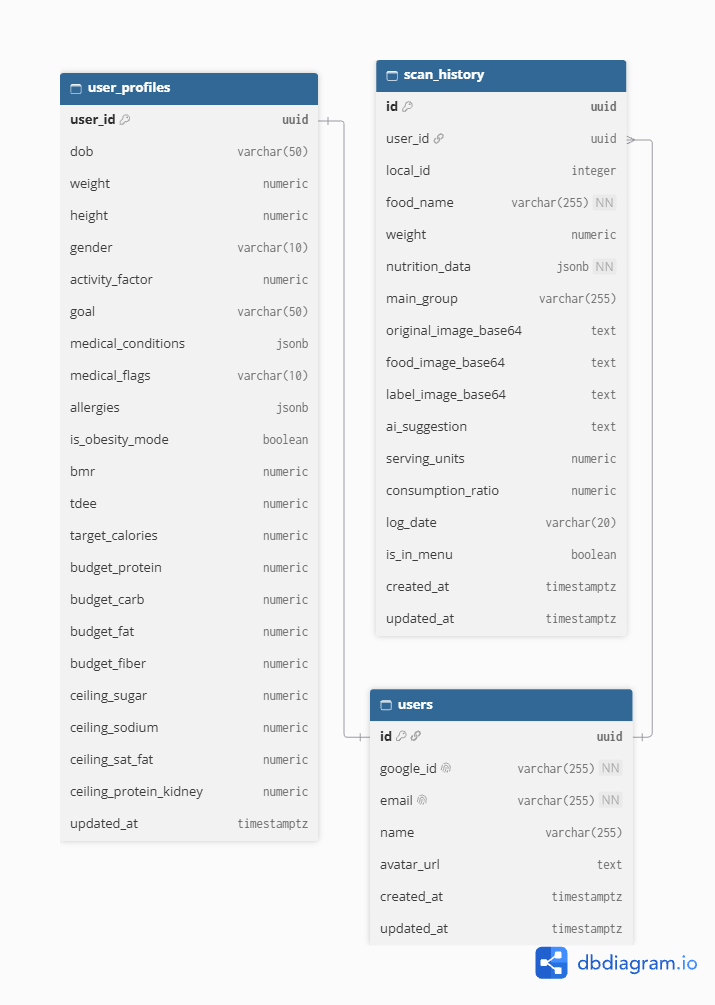
\includegraphics[width=0.82\textwidth,height=0.58\textheight,keepaspectratio]{so_do_co_so_du_lieu.png}
    \caption{Sơ đồ tổ chức cơ sở dữ liệu quan hệ và bảng tham chiếu dinh dưỡng của NutriCare}
    \label{fig:database_schema}
\end{figure}

\begin{itemize}[leftmargin=0.8cm, label=\textbullet, itemsep=2.5pt, topsep=2pt]
    \item \textbf{Bảng tham chiếu dinh dưỡng tĩnh:} Gồm $84$ dòng nguyên liệu chuẩn hóa (chủ yếu ở trạng thái tươi sống nguyên bản, kèm hạt hạnh nhân và óc chó rang) với $206$ cột giá trị và đơn vị dưỡng chất trên $100\text{ g}$ phần ăn được, ánh xạ từ $50$ nhãn nhận diện kèm thông tin chi tiết từng bộ phận thực phẩm.
    \item \textbf{Bảng Tài khoản người dùng (trên máy chủ):} Lưu mã định danh duy nhất của hệ thống, mã liên kết Google, thư điện tử, họ tên và đường dẫn ảnh đại diện.
    \item \textbf{Bảng Hồ sơ sức khỏe:} Liên kết $1\text{--}1$ với tài khoản, lưu ngày sinh, cân nặng, chiều cao, giới tính, mức độ vận động, mục tiêu dinh dưỡng, danh sách dị ứng, 6 bệnh lý mạn tính (kèm mã cờ nhị phân 6-bit), trạng thái bật chế độ kiểm soát béo phì cùng các ngưỡng tính sẵn (chỉ số chuyển hóa cơ bản, tổng tiêu hao năng lượng, calo mục tiêu, định mức chất đa lượng và giới hạn an toàn y khoa).
    \item \textbf{Bảng Nhật ký tra cứu thực phẩm:} Liên kết $1\text{--}N$ với tài khoản, lưu tên món chuẩn hóa, khối lượng trên tem nhãn, số phần chuẩn quy đổi, tỷ lệ tiêu thụ $\gamma$, ngày ăn, cờ đánh dấu món có thuộc thực đơn ngày hay không, bản chụp toàn bộ bảng dưỡng chất của lần quét đó, ảnh món ăn (đường dẫn tệp trên máy và dữ liệu ảnh nén đồng bộ), nội dung tư vấn AI và mã ánh xạ thứ tự bản ghi giữa điện thoại với máy chủ.
\end{itemize}

Thiết kế cơ sở dữ liệu này giải quyết ba vấn đề thực tế quan trọng khi vận hành ứng dụng lâu dài:
\begin{enumerate}[leftmargin=0.8cm, itemsep=2.5pt, topsep=2pt]
    \item \textbf{Đạt chuẩn chuẩn hóa 2NF và đóng băng dữ liệu lịch sử:} Cả ba bảng quan hệ đều dùng khóa chính đơn thuộc tính, bảo đảm mọi thông tin chi tiết phụ thuộc hoàn toàn vào khóa chính. Quan trọng hơn, mỗi bản ghi quét tự lưu riêng một bản sao bất biến của thành phần dinh dưỡng ngay tại thời điểm tra cứu thay vì chỉ lưu mã trỏ sang bảng tĩnh. Nhờ đó, khi bảng tham chiếu được bổ sung thực phẩm mới hoặc hiệu chỉnh số liệu về sau, toàn bộ lịch sử tiêu thụ và kết quả đánh giá sức khỏe trước đây của người dùng vẫn giữ nguyên độ chính xác.
    \item \textbf{Tách biệt Lịch sử tra cứu và Thực đơn ngày:} Mọi lần quét mới đều lưu tự động vào lịch sử với trạng thái chưa thuộc thực đơn ngày. Chỉ khi người dùng chủ động nhấn thêm món vào thực đơn hôm nay (tính năng dành cho tài khoản đã đăng nhập), bản ghi mới được cộng dồn vào tiến trình dinh dưỡng của ngày tương ứng; ngược lại, khi gỡ khỏi thực đơn ngày, bản ghi vẫn được giữ lại trong lịch sử.
    \item \textbf{Tránh ghi đè dữ liệu khi gộp lịch sử Khách:} Khi sử dụng ở chế độ Khách, các bản ghi trên điện thoại được SQLite đánh số thứ tự tự động từ $1$, rất dễ trùng với mã thứ tự bản ghi cũ đã lưu sẵn trên máy chủ của tài khoản. Vì vậy, khi người dùng đăng nhập và khôi phục dữ liệu từ đám mây, hệ thống kiểm tra những bản ghi khách chưa đồng bộ bị trùng mã thứ tự và cấp lại số thứ tự mới lớn hơn trước khi đẩy lên máy chủ, bảo đảm gộp đầy đủ hai nguồn dữ liệu mà không làm mất lịch sử cũ.
\end{enumerate}

\section{Các luồng xử lý cốt lõi của hệ thống}
\label{sec:core-pipelines}

Hoạt động của NutriCare xoay quanh ba luồng xử lý chính: nhận diện thực phẩm kết hợp đọc khối lượng từ tem nhãn, đánh giá luật dinh dưỡng y khoa kèm tư vấn AI, và quản lý xác thực -- đồng bộ giữa chế độ Khách với tài khoản Google.

\subsection{Luồng nhận diện thực phẩm và đọc khối lượng từ tem nhãn}
\label{subsec:multimodal-pipeline}

Kế thừa mô hình định vị YOLO26s và phân hệ nhận dạng văn bản đã nêu ở Mục~\ref{sec:yolo-object-detection} và Mục~\ref{sec:mlkit-ocr}, ứng dụng triển khai quy trình xử lý ảnh trực tiếp trên điện thoại qua bốn bước (Hình~\ref{fig:multimodal_pipeline}):

\begin{figure}[htbp]
    \centering
    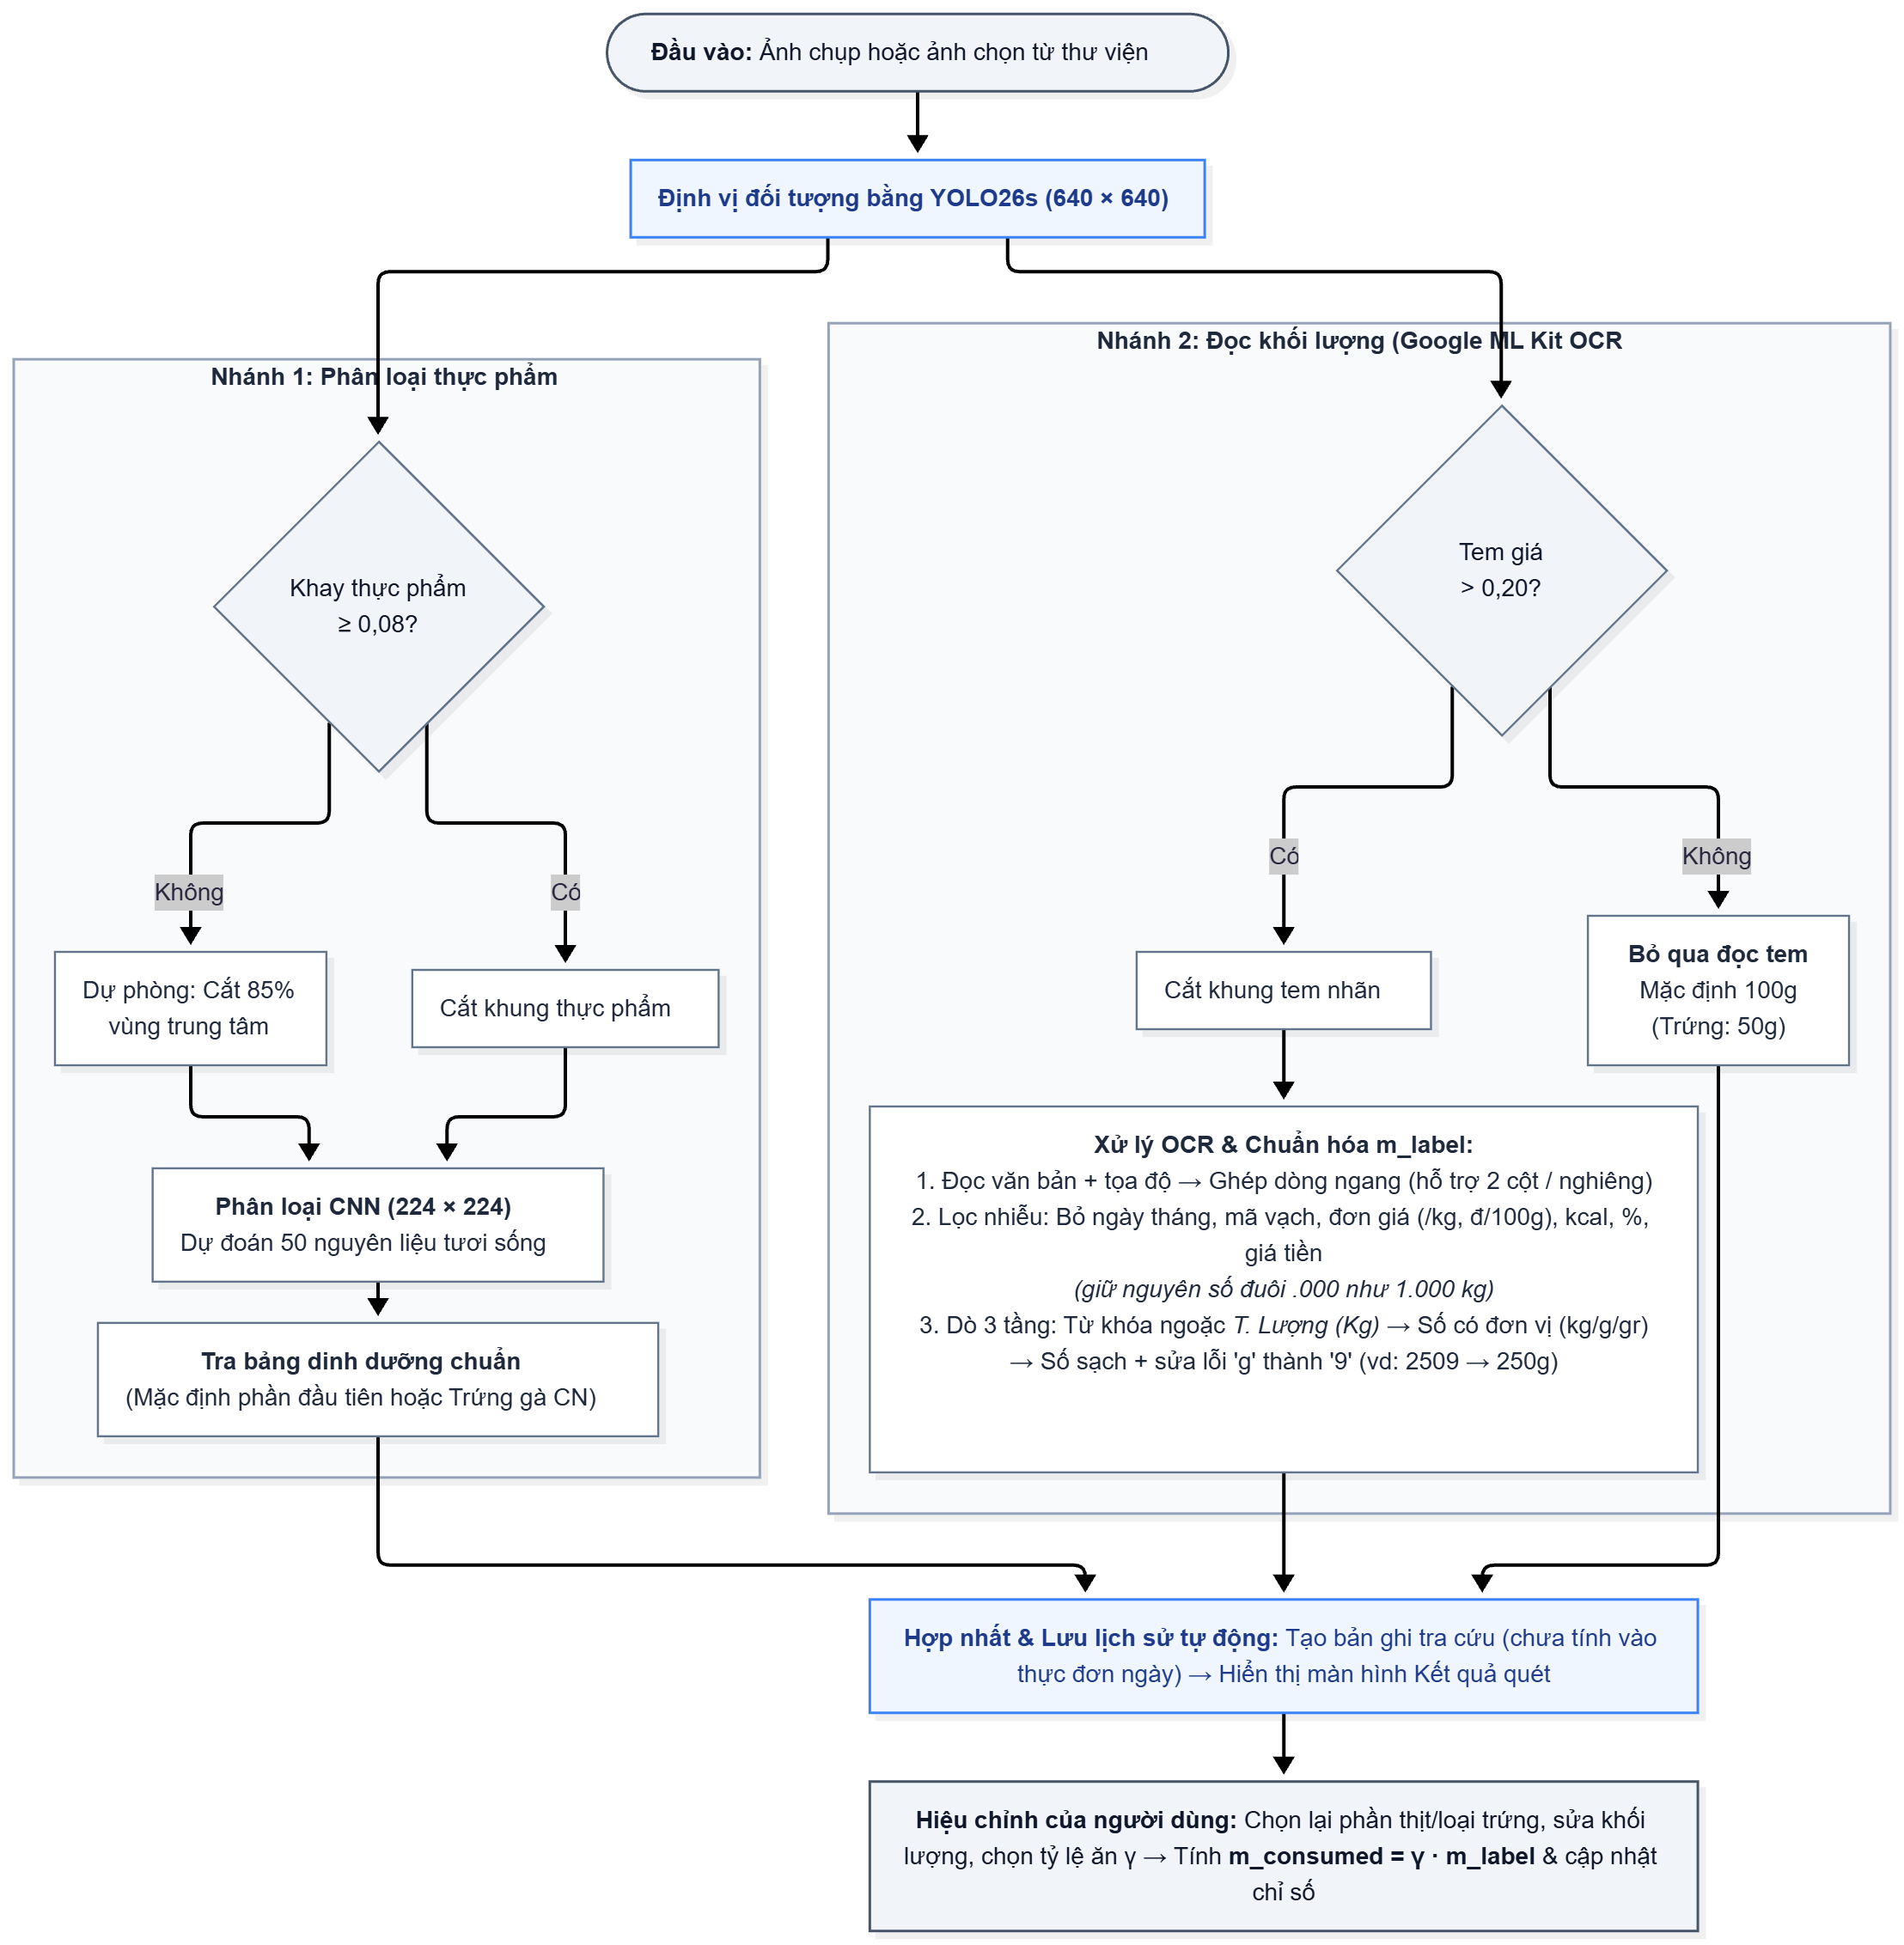
\includegraphics[width=0.95\textwidth,height=0.62\textheight,keepaspectratio]{so_do_luong_du_lieu_da_mo_hinh.png}
    \caption{Luồng xử lý nhận diện thực phẩm bằng YOLO26s, CNN 50 lớp và đọc khối lượng trên tem nhãn}
    \label{fig:multimodal_pipeline}
\end{figure}

\begin{enumerate}[leftmargin=0.8cm, itemsep=2.5pt, topsep=2pt]
    \item \textbf{Định vị vùng khay thực phẩm và vùng tem giá (YOLO26s):} Ảnh đầu vào được đưa về kích thước $640 \times 640$ điểm ảnh (chuẩn hóa giá trị màu về khoảng $[0;\ 1]$) để mô hình YOLO26s tìm đồng thời vùng chứa thực phẩm và vùng tem cân. Với vùng thực phẩm, hệ thống áp dụng ngưỡng tin cậy tối thiểu $0{,}08$; nếu ảnh quá mờ hoặc góc chụp lệch khiến mô hình không đạt ngưỡng, cơ chế dự phòng sẽ tự động cắt lấy $85\%$ vùng trung tâm ảnh để quy trình không bị gián đoạn. Vùng tem giá được cắt riêng khi vượt ngưỡng tin cậy $0{,}20$.
    \item \textbf{Phân loại nguyên liệu (CNN):} Vùng ảnh thực phẩm sau khi cắt được co dãn về kích thước $224 \times 224$ điểm ảnh (giữ dải màu gốc $0\text{--}255$) và truyền qua mô hình phân loại 50 nguyên liệu tươi sống. Nếu kết quả nhận diện là \textit{Trứng}, hệ thống tự động gắn với nhóm 4 loại trứng phổ biến và chọn mặc định là \textit{Trứng gà công nghiệp} ($50\text{ g}$/quả) khi chưa có khối lượng từ tem nhãn.
    \item \textbf{Trích xuất khối lượng bằng thuật toán đọc tem theo không gian (Google ML Kit):} Dữ liệu văn bản thu từ ảnh tem giá đi kèm tọa độ khung bao của từng dòng chữ được xử lý qua ba bước lọc nhằm khắc phục nhược điểm của tem siêu thị:
    \begin{itemize}[leftmargin=0.6cm, label=--, itemsep=1.5pt, topsep=1.5pt]
        \item \textit{Ghép dòng theo hàng ngang trực quan:} Nhiều tem cân in dạng bảng 2 cột (cột trái ghi tiêu đề như ``T. Lượng (Kg):'', cột phải ghi số ``0.308'') hoặc ảnh chụp hơi nghiêng khiến bộ đọc chữ tách rời nhãn với giá trị. Thuật toán so sánh tọa độ tâm theo chiều dọc để ghép các ô cùng hàng ngang thành một dòng hoàn chỉnh trước khi phân tích.
        \item \textit{Loại bỏ nhiễu có chủ đích:} Hệ thống lọc bỏ ngày đóng gói, hạn sử dụng, chuỗi mã vạch dài, đơn giá trên khối lượng (như \texttt{đ/100g}, \texttt{/kg}), chỉ số năng lượng (\texttt{kcal}), phần trăm và giá tiền đi kèm từ khóa (\textit{Đơn giá, Thành tiền, vnđ}). Đặc biệt, ứng dụng không xóa mù các cụm số đuôi \texttt{.000}, nhờ đó loại chính xác giá tiền (như $121{.}000\text{ vnđ}$) mà vẫn giữ toàn vẹn những tem cân ghi khối lượng dạng $1{.}000\text{ kg}$ hay $1{.}00\text{ kg}$.
        \item \textit{Dò tìm khối lượng theo 3 tầng ưu tiên:} Trước tiên tìm các dòng chứa từ khóa khối lượng (\textit{Khối lượng, Trọng lượng, T. Lượng, KL, TL, Net Wt} --- loại trừ chữ ``lượng'' đứng riêng để tránh nhầm với năng lượng) và nhận diện luôn đơn vị đặt trong ngoặc của tiêu đề; nếu không có từ khóa mới xét tới số có kèm đơn vị đo tường minh (\texttt{kg, g, gr, gram}); cuối cùng mới kiểm tra số đơn lẻ sạch kèm quy tắc sửa lỗi hay gặp khi bộ đọc chữ nhận nhầm chữ \texttt{g} thành số \texttt{9} ở cuối (chẳng hạn \texttt{2509} thành $250\text{ g}$). Nếu không có tem nhãn, hệ thống gán giá trị tạm $100\text{ g}$.
    \end{itemize}
    \item \textbf{Tra cứu bảng chuẩn và hiệu chỉnh khẩu phần thực tế $\gamma$:} Tên nguyên liệu được ánh xạ vào bảng dinh dưỡng $84$ dòng $\times$ $206$ cột. Trên màn hình kết quả, người dùng có thể đổi phần thịt cụ thể hoặc chọn lại loại trứng, sửa khối lượng nhãn $m_{\text{label}}$ và chọn tỷ lệ ăn thực tế $\gamma$ (theo các mức $25\%\text{--}100\%$, nhập số gam/phần trăm tùy ý hoặc số quả trứng) để tính lượng thực ăn $m_{\text{consumed}}$ theo Phương trình~\eqref{eq:consumed-mass}.
\end{enumerate}

\subsection{Bộ luật dinh dưỡng y khoa ba lớp và tư vấn AI}
\label{subsec:medical-rule-engine}

Các công thức và ngưỡng khuyến nghị y khoa từ Mục~\ref{sec:nutrition-foundation} được hiện thực hóa trên ứng dụng qua ba lớp kiểm soát nối tiếp nhau (chỉ mở khóa khi người dùng đã đăng nhập, Hình~\ref{fig:medical_rule_engine}):

\begin{figure}[htbp]
    \centering
    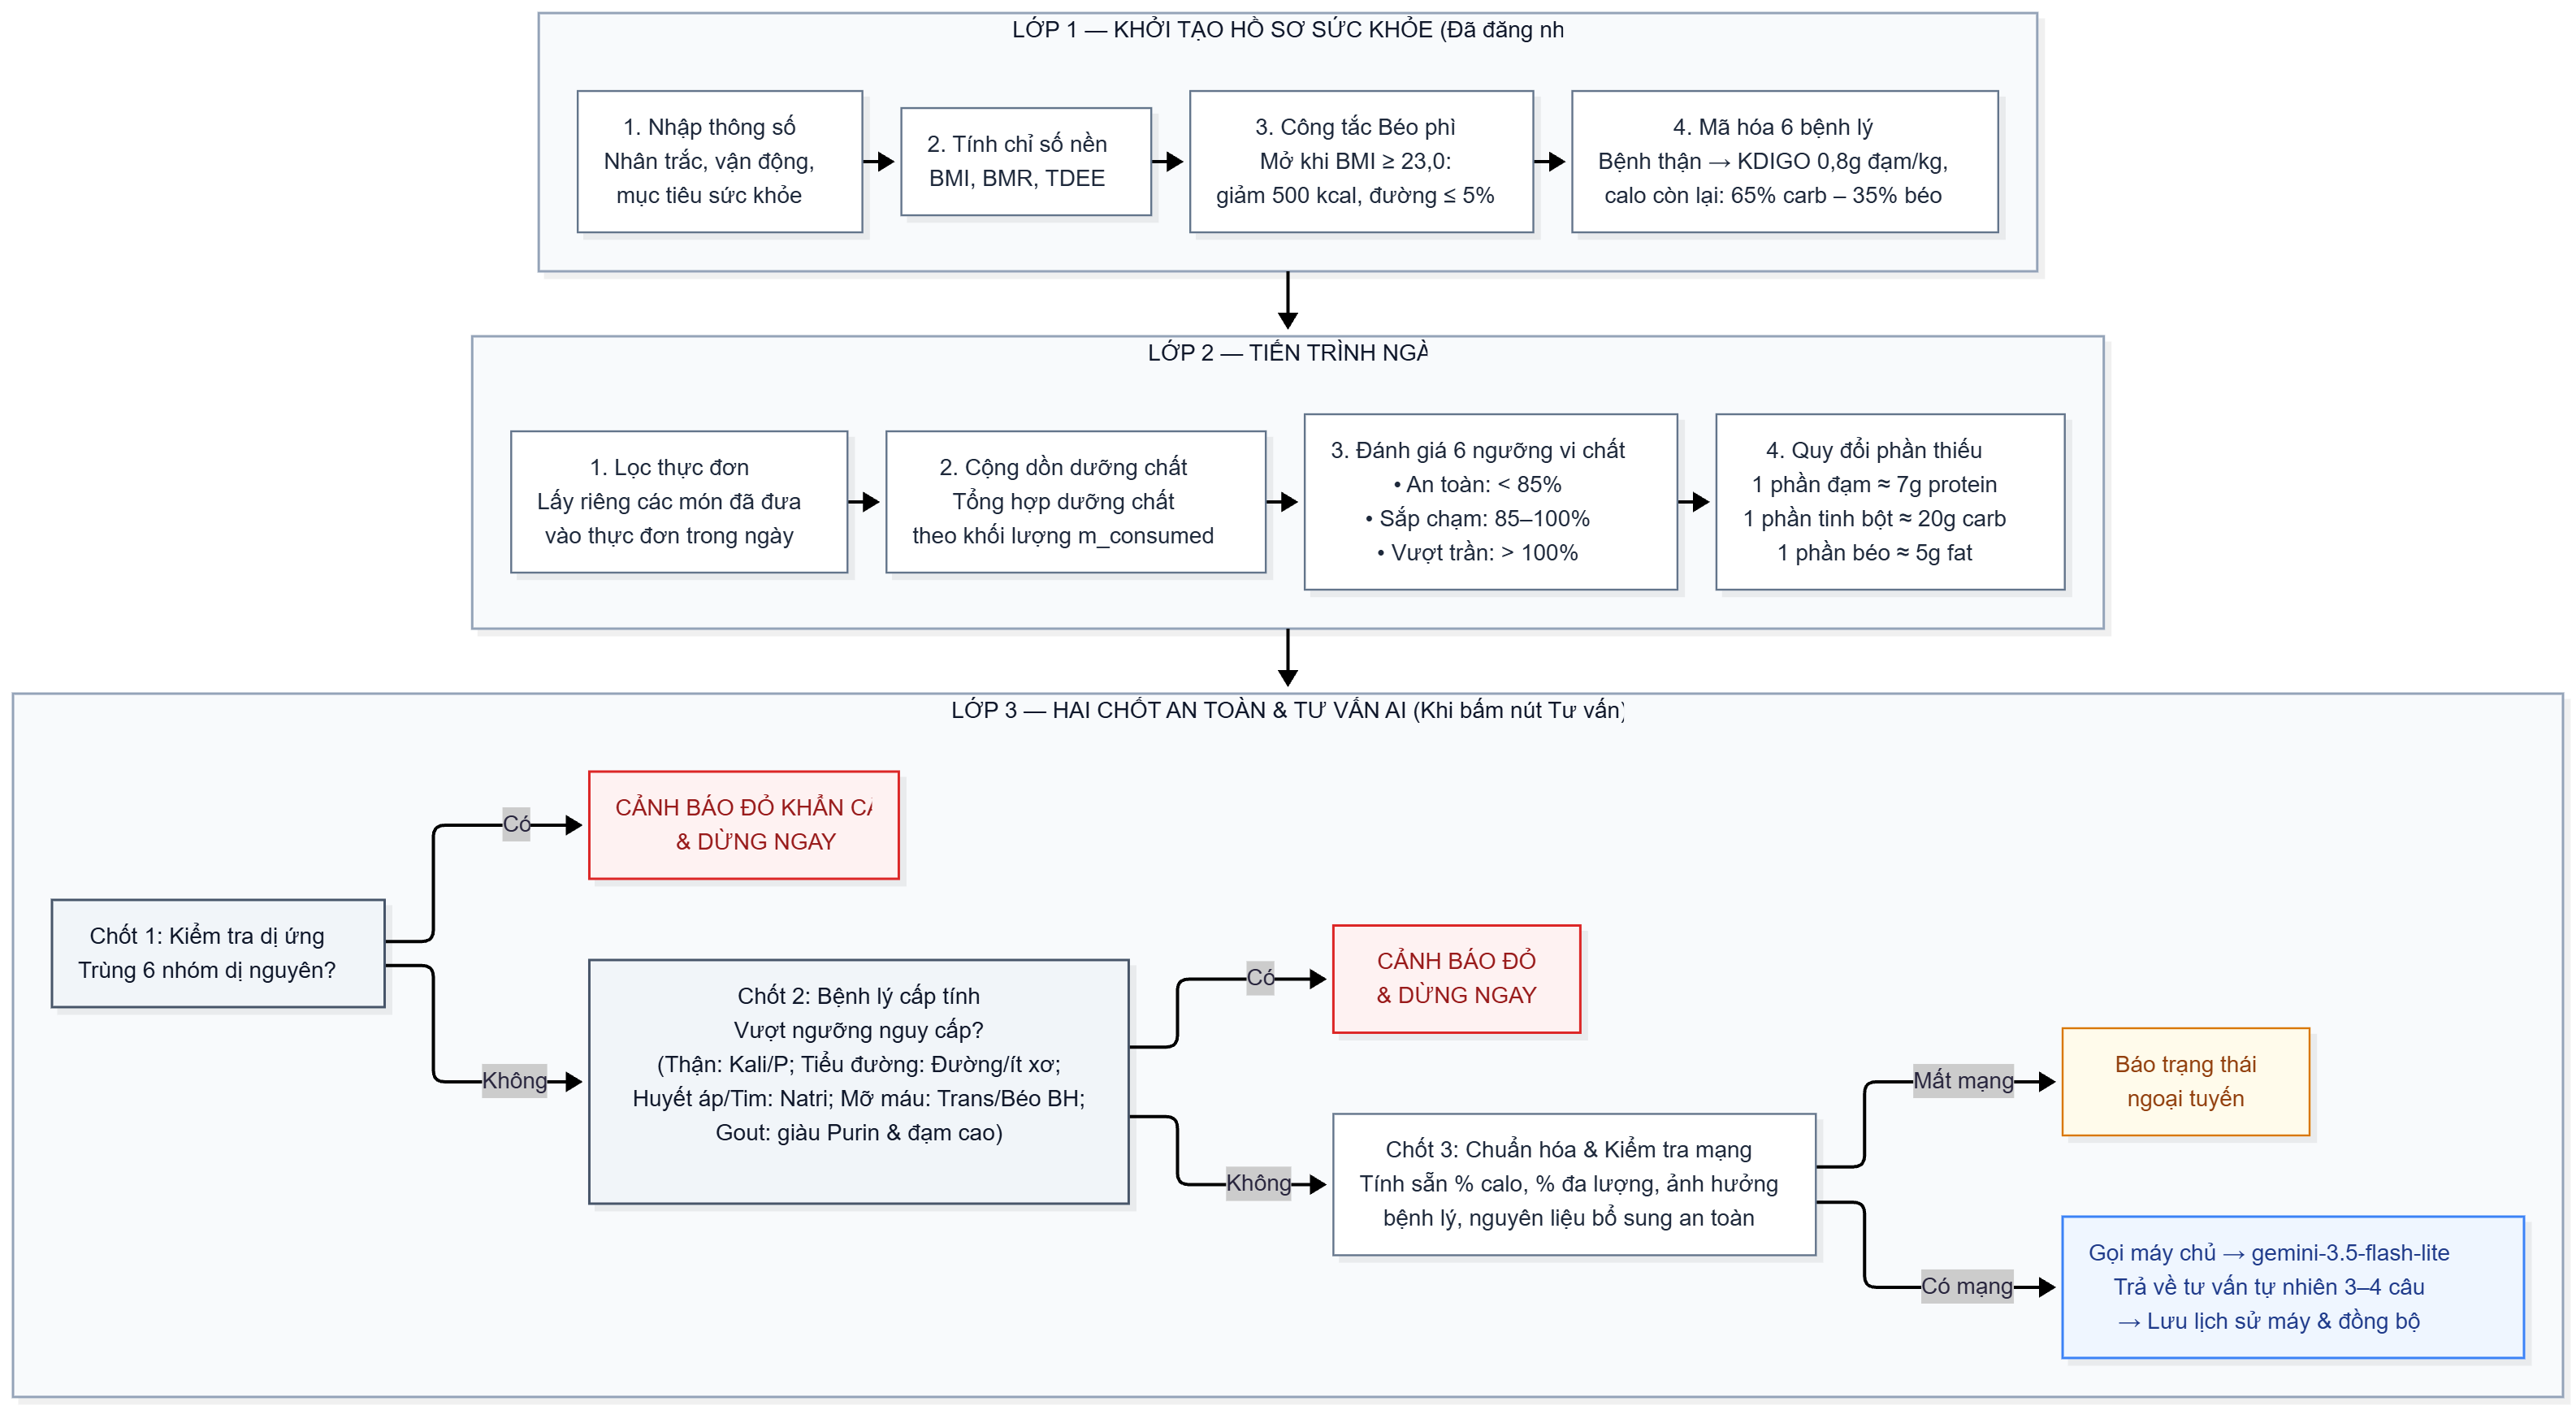
\includegraphics[width=0.98\textwidth,height=0.45\textheight,keepaspectratio]{so_do_cong_cu_luat_y_khoa.png}
    \caption[Lưu đồ bộ luật dinh dưỡng y khoa ba lớp và tư vấn AI]{Lưu đồ thực thi bộ luật dinh dưỡng y khoa ba lớp, chốt chặn an toàn và mô hình \nolinkurl{gemini-3.5-flash-lite}}
    \label{fig:medical_rule_engine}
\end{figure}

\begin{enumerate}[leftmargin=0.8cm, itemsep=2.5pt, topsep=2pt]
    \item \textbf{Lớp 1 -- Tính toán hồ sơ cá nhân:} Sau khi người dùng nhập thông số cơ thể, ứng dụng tính $\mathrm{BMI}$, chuyển hóa cơ bản, nhu cầu năng lượng ngày và mã hóa 6 bệnh lý mạn tính thành chuỗi cờ nhị phân. Công tắc \textit{Chế độ kiểm soát béo phì} chỉ cho phép bật khi $\mathrm{BMI} \ge 23{,}0$; khi bật, mục tiêu tự động đặt là giảm cân (thâm hụt $500\text{ kcal/ngày}$ theo cơ cấu $30\%$ đạm -- $40\%$ tinh bột -- $30\%$ chất béo) và hạ trần đường tự do từ $10\%$ xuống $5\%$ tổng năng lượng. Nếu người dùng mắc bệnh thận mạn, hệ thống áp dụng ngưỡng đạm $0{,}8\text{ g/kg/ngày}$ theo KDIGO rồi chia phần năng lượng còn lại theo tỷ lệ $65\%$ tinh bột và $35\%$ chất béo.
    \item \textbf{Lớp 2 -- Theo dõi tiến trình ngày và quy đổi phần ăn thiếu hụt:} Hệ thống chỉ lọc các món đã đưa vào thực đơn của ngày đang xem để cộng dồn năng lượng, 4 chất đa lượng và 6 ngưỡng vi chất (\textit{Natri, Kali, Photpho, Đường tự do, Chất béo bão hòa, Trần đạm bệnh thận}), đồng thời hiển thị cảnh báo theo 3 mức màu (\textit{An toàn} khi dưới $85\%$, \textit{Sắp chạm ngưỡng} từ $85\%$ đến $100\%$, và \textit{Vượt trần} khi trên $100\%$). Lượng thiếu hụt $R_j$ từ Phương trình~\eqref{eq:daily-remaining} được quy đổi theo Phương trình~\eqref{eq:servings-needed} thành ba chỉ số gợi ý dễ hiểu: \textbf{1 phần đạm $\approx 7\text{ g}$ protein}, \textbf{1 phần tinh bột $\approx 20\text{ g}$ carb} và \textbf{1 phần béo $\approx 5\text{ g}$ fat}.
    \item \textbf{Lớp 3 -- Hai chốt chặn an toàn tuyệt đối trước khi gọi AI:} Khi người dùng bấm yêu cầu tư vấn cho một khẩu phần cụ thể, ứng dụng kiểm tra lần lượt:
    \begin{itemize}[leftmargin=0.6cm, label=--, itemsep=1.5pt, topsep=1.5pt]
        \item \textit{Chốt 1 (Kiểm tra dị ứng):} Đối chiếu thực phẩm với 6 nhóm dị nguyên đã khai báo; nếu trùng khớp, hiển thị ngay cảnh báo đỏ nghiêm cấm sử dụng và ngắt luồng gọi AI.
        \item \textit{Chốt 2 (Kiểm tra ngưỡng bệnh lý cấp tính trên khẩu phần $m_{\text{consumed}}$):} Ngắt luồng và cảnh báo không nên dùng ngay trên điện thoại nếu món ăn vượt ngưỡng nguy hiểm (Bệnh thận: $\mathrm{Kali} \ge 600\text{ mg}$ hoặc $\mathrm{Photpho} \ge 400\text{ mg}$; Đái tháo đường: $\mathrm{Đường} \ge 50\%$ trần ngày và $\mathrm{Chất\ xơ} < 1\text{ g}$; Tăng huyết áp hoặc tim mạch: $\mathrm{Natri} \ge 50\%$ trần ngày hoặc từ $1000\text{ mg}$ trở lên; Mỡ máu: chất béo chuyển hóa từ $0{,}5\text{ g}$ hoặc chất béo bão hòa đạt từ $50\%$ trần ngày; Bệnh gút: thực phẩm giàu nhân purin có lượng đạm từ $35\text{ g}$ trở lên).
        \item \textit{Chốt 3 (Chuẩn hóa số liệu và gọi \nolinkurl{gemini-3.5-flash-lite}):} Khi khẩu phần vượt qua hai chốt chặn an toàn, điện thoại tự tính sẵn tỷ lệ phần trăm calo, tỷ lệ đa lượng đóng góp, mức độ ảnh hưởng lên từng bệnh lý và danh sách nguyên liệu tươi sống bổ sung không gây dị ứng rồi mới gửi gói dữ liệu sang máy chủ để mô hình \nolinkurl{gemini-3.5-flash-lite} diễn giải thành lời khuyên hoàn chỉnh (hoặc thông báo ngoại tuyến an toàn nếu mất kết nối mạng).
    \end{itemize}
\end{enumerate}

\subsection{Luồng xác thực, chế độ Khách và đồng bộ đám mây}
\label{subsec:auth-sync-flow}

Quy trình quản lý phiên và đồng bộ dữ liệu được thiết kế để chuyển đổi mượt mà giữa dùng ngoại tuyến không cần tài khoản và sao lưu đám mây (Hình~\ref{fig:auth_sync_flow}).

\begin{figure}[htbp]
    \centering
    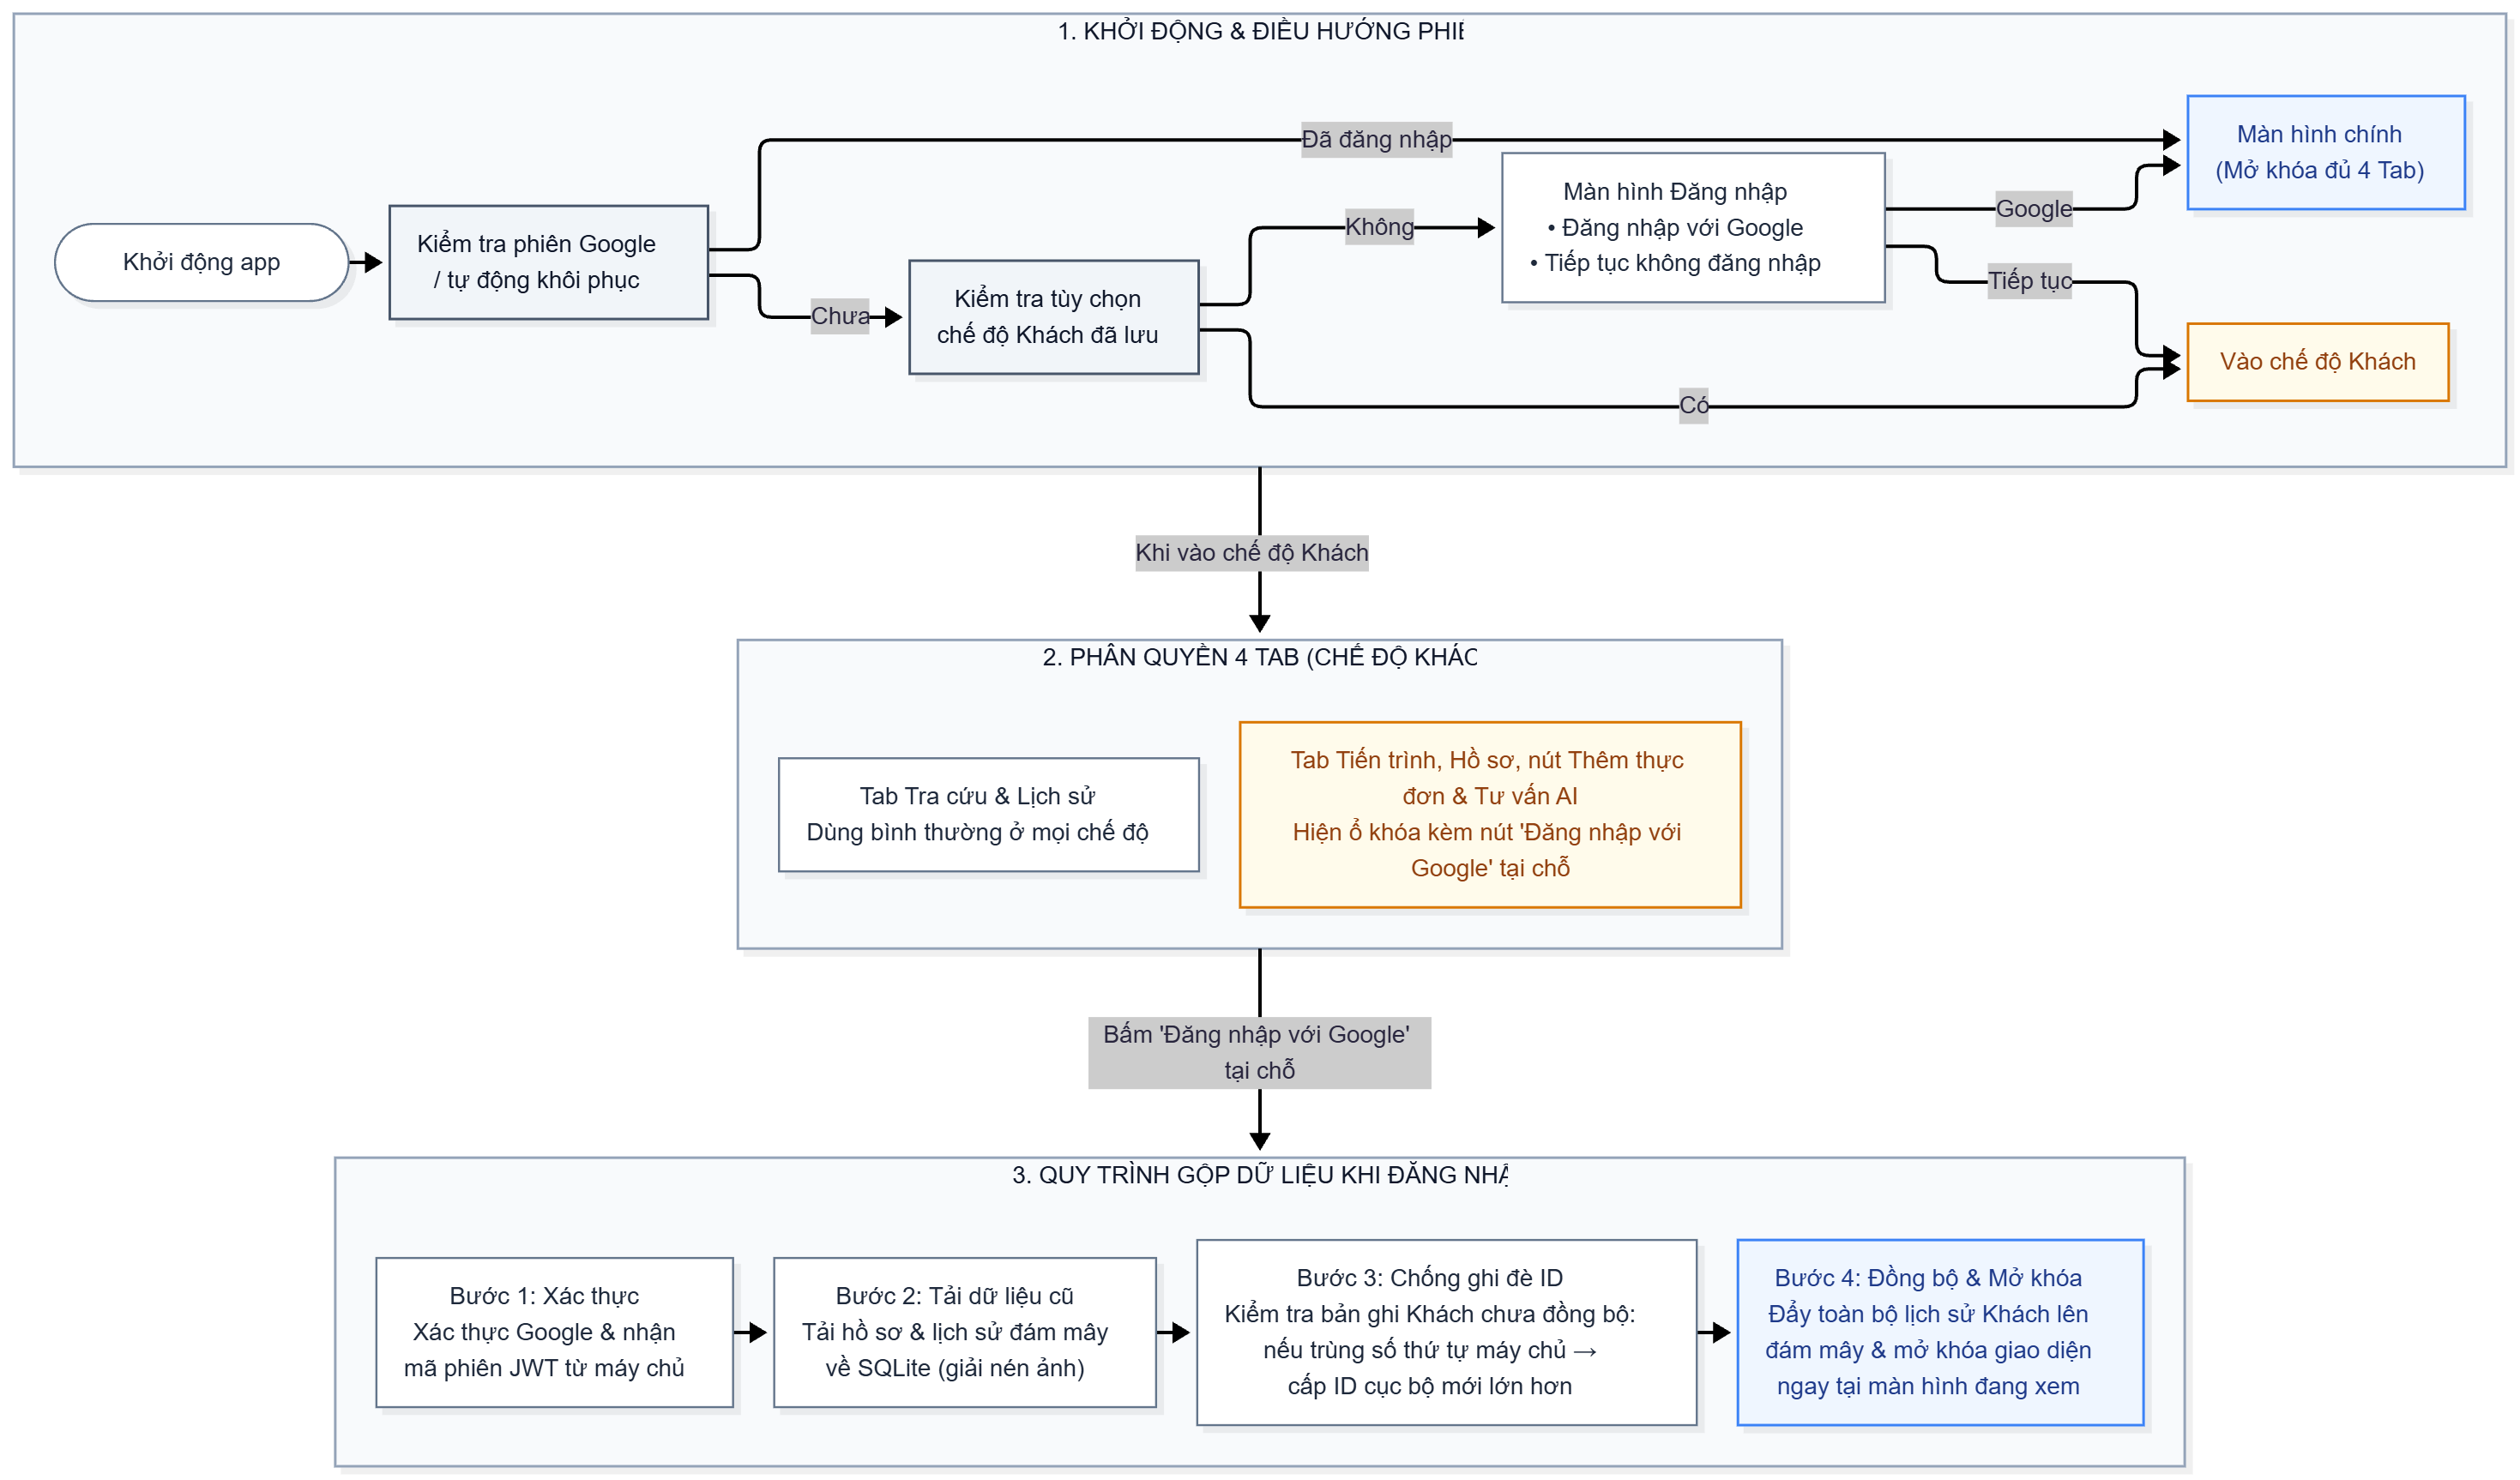
\includegraphics[width=0.98\textwidth,height=0.45\textheight,keepaspectratio]{so_do_xac_thuc_dong_bo_khach.png}
    \caption{Lưu đồ xác thực, sử dụng ở chế độ Khách và gộp dữ liệu khi đăng nhập Google}
    \label{fig:auth_sync_flow}
\end{figure}

Khi mở ứng dụng, hệ thống kiểm tra phiên đăng nhập đã lưu (hoặc thử tự động khôi phục phiên Google ngầm). Nếu chưa đăng nhập nhưng người dùng từng chọn dùng thử ở chế độ Khách trước đó, ứng dụng vào thẳng màn hình chính thay vì hỏi đăng nhập lại; ngược lại sẽ mở màn hình đăng nhập với hai lựa chọn là \textit{Đăng nhập với Google} hoặc \textit{Tiếp tục không cần đăng nhập}.

Với tài khoản đã đăng nhập, mọi thay đổi trên hồ sơ, tỷ lệ ăn hoặc nội dung tư vấn AI đều được tự động sao lưu ngầm lên máy chủ PostgreSQL sau khoảng trễ ngắn $0{,}5\text{ giây}$ để gom các thao tác liên tiếp của người dùng. Trường hợp người dùng bắt đầu ở chế độ Khách rồi mới bấm đăng nhập Google ngay trên màn hình kết quả hay mục đang khóa, hệ thống thực hiện tuần tự bốn bước: xác thực Google và nhận mã phiên từ máy chủ; tải hồ sơ và lịch sử cũ trên đám mây về SQLite (kèm giải nén các ảnh Base64 thành tệp cục bộ); cấp lại mã thứ tự mới cho các bản ghi Khách chưa đồng bộ bị trùng mã với đám mây; rồi đẩy toàn bộ lịch sử Khách lên máy chủ và mở khóa giao diện ngay tại màn hình hiện tại. Khi người dùng đăng xuất chủ động, hệ thống cảnh báo nếu còn dữ liệu chưa kịp sao lưu và dọn sạch cơ sở dữ liệu cục bộ để bảo mật thông tin.

\section{Thiết kế giao diện ứng dụng di động}
\label{sec:ui-design}

Giao diện NutriCare sử dụng tông xanh lá chủ đạo kết hợp hệ thống màu cảnh báo y khoa (xanh an toàn, cam lưu ý, đỏ nguy hiểm) và xoay quanh thanh điều hướng 4 mục cố định ở đáy màn hình. Hình~\ref{fig:ui_auth_scan} minh họa màn hình khởi đầu cho phép lựa chọn đăng nhập hoặc dùng ở chế độ Khách cùng màn hình quét ảnh thực phẩm chính.

\begin{figure}[htbp]
    \centering
    {\setlength{\fboxsep}{0pt}\setlength{\fboxrule}{0.4pt}%
    \begin{minipage}[b]{0.46\textwidth}
        \centering
        \fcolorbox{black!15}{white}{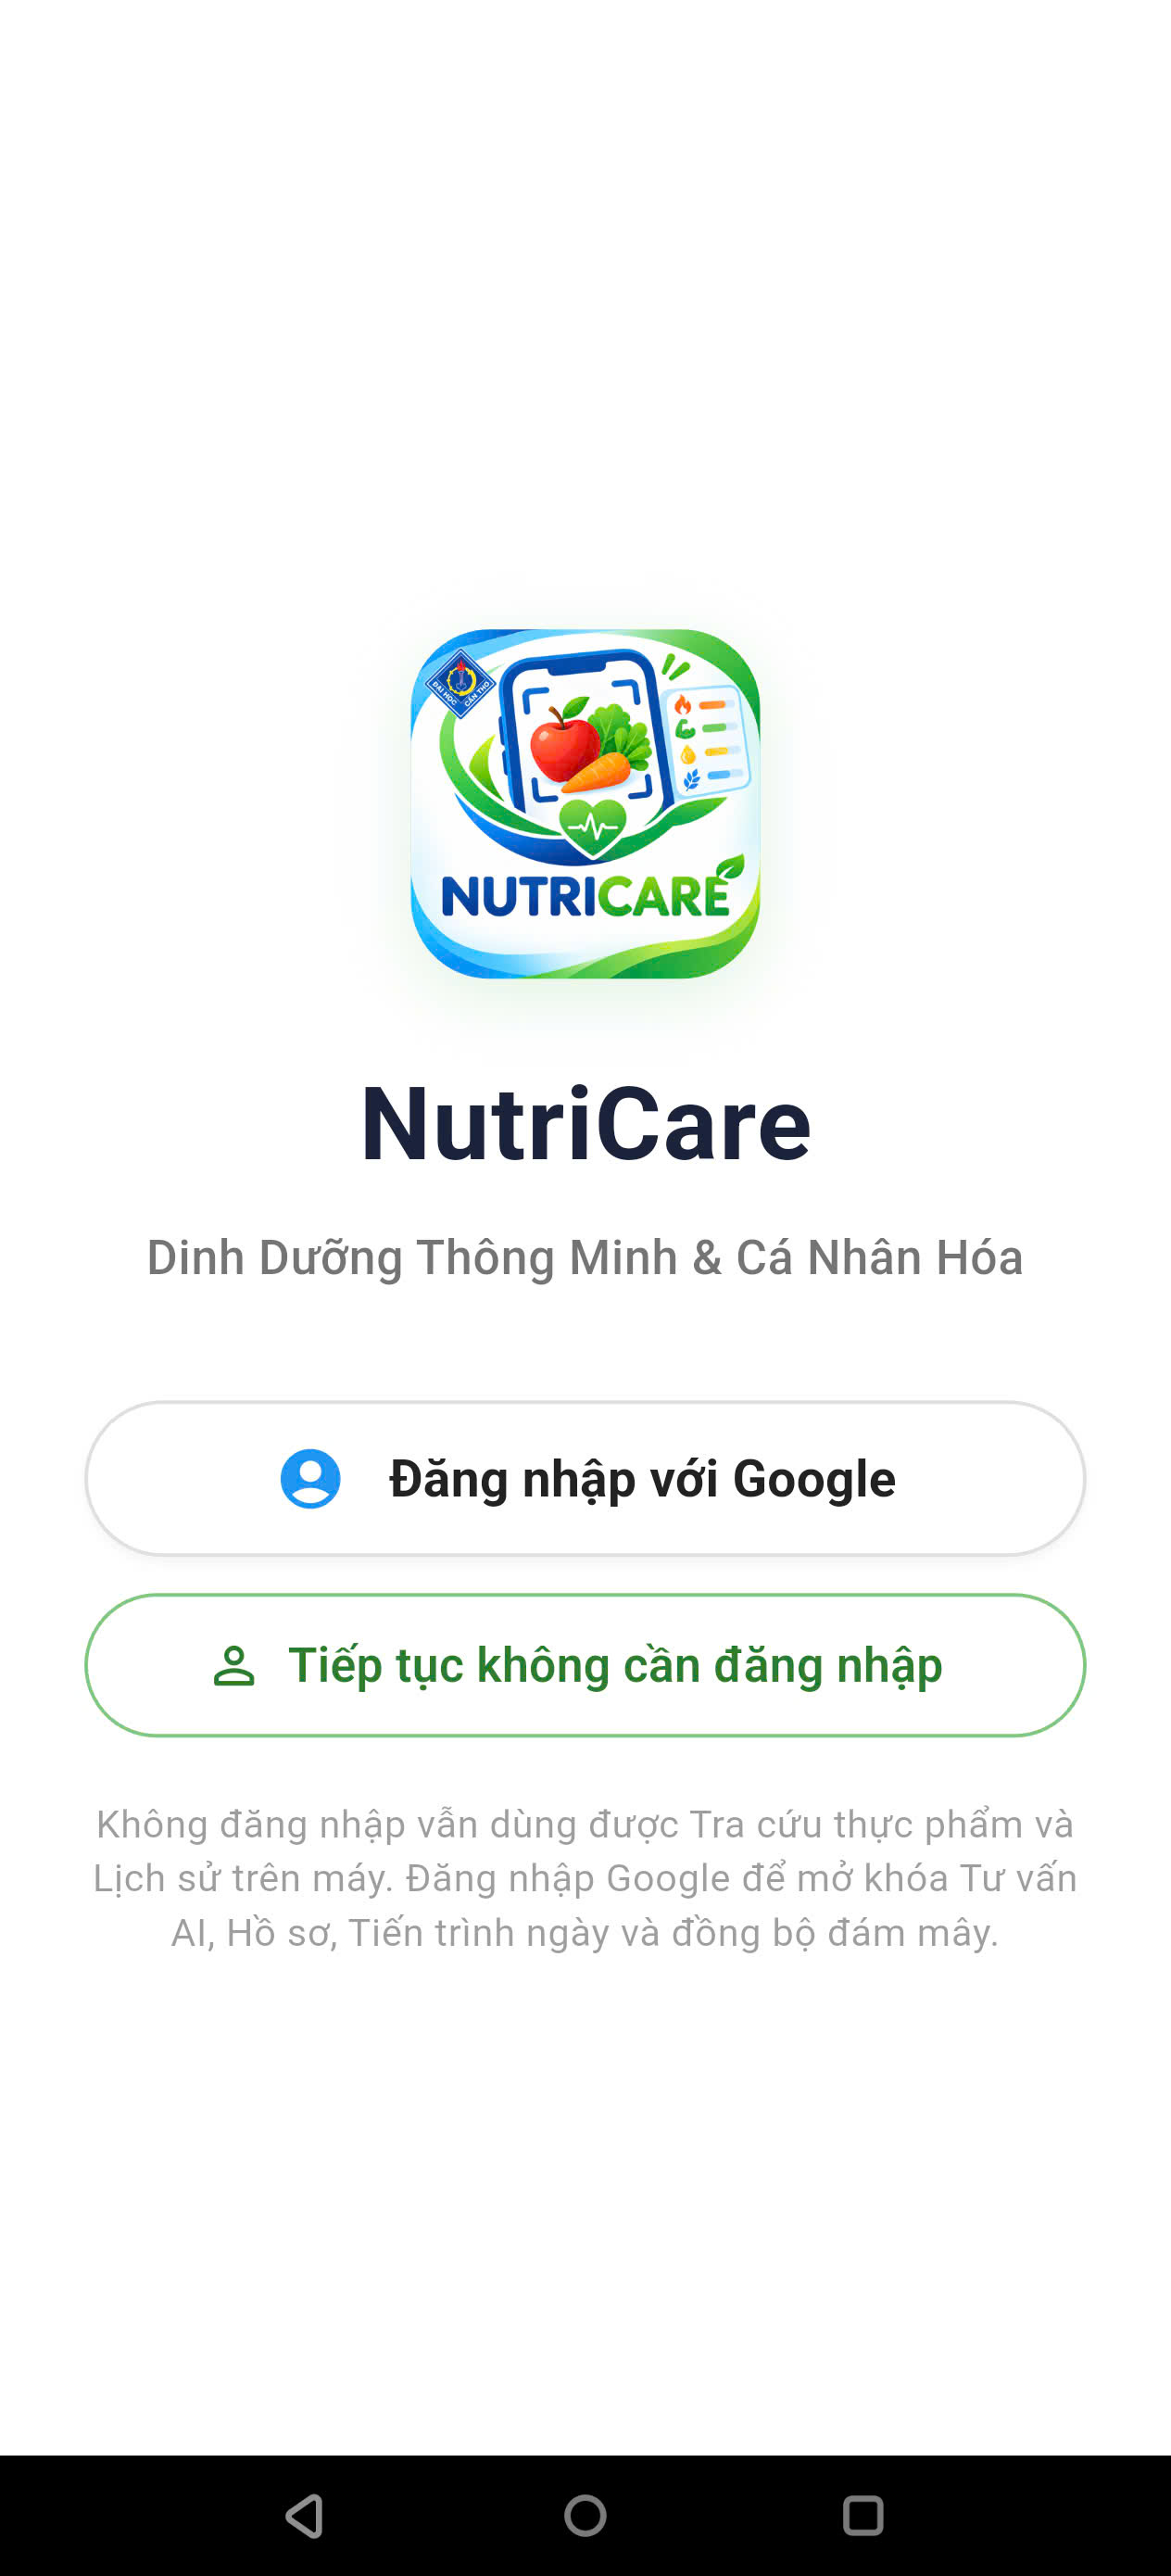
\includegraphics[width=0.88\textwidth,height=0.46\textheight,keepaspectratio]{hinh3_1_dang_nhap.jpg}}
        \par\vspace{4pt}{\small (a) Màn hình Đăng nhập}
    \end{minipage}
    \hfill
    \begin{minipage}[b]{0.46\textwidth}
        \centering
        \fcolorbox{black!15}{white}{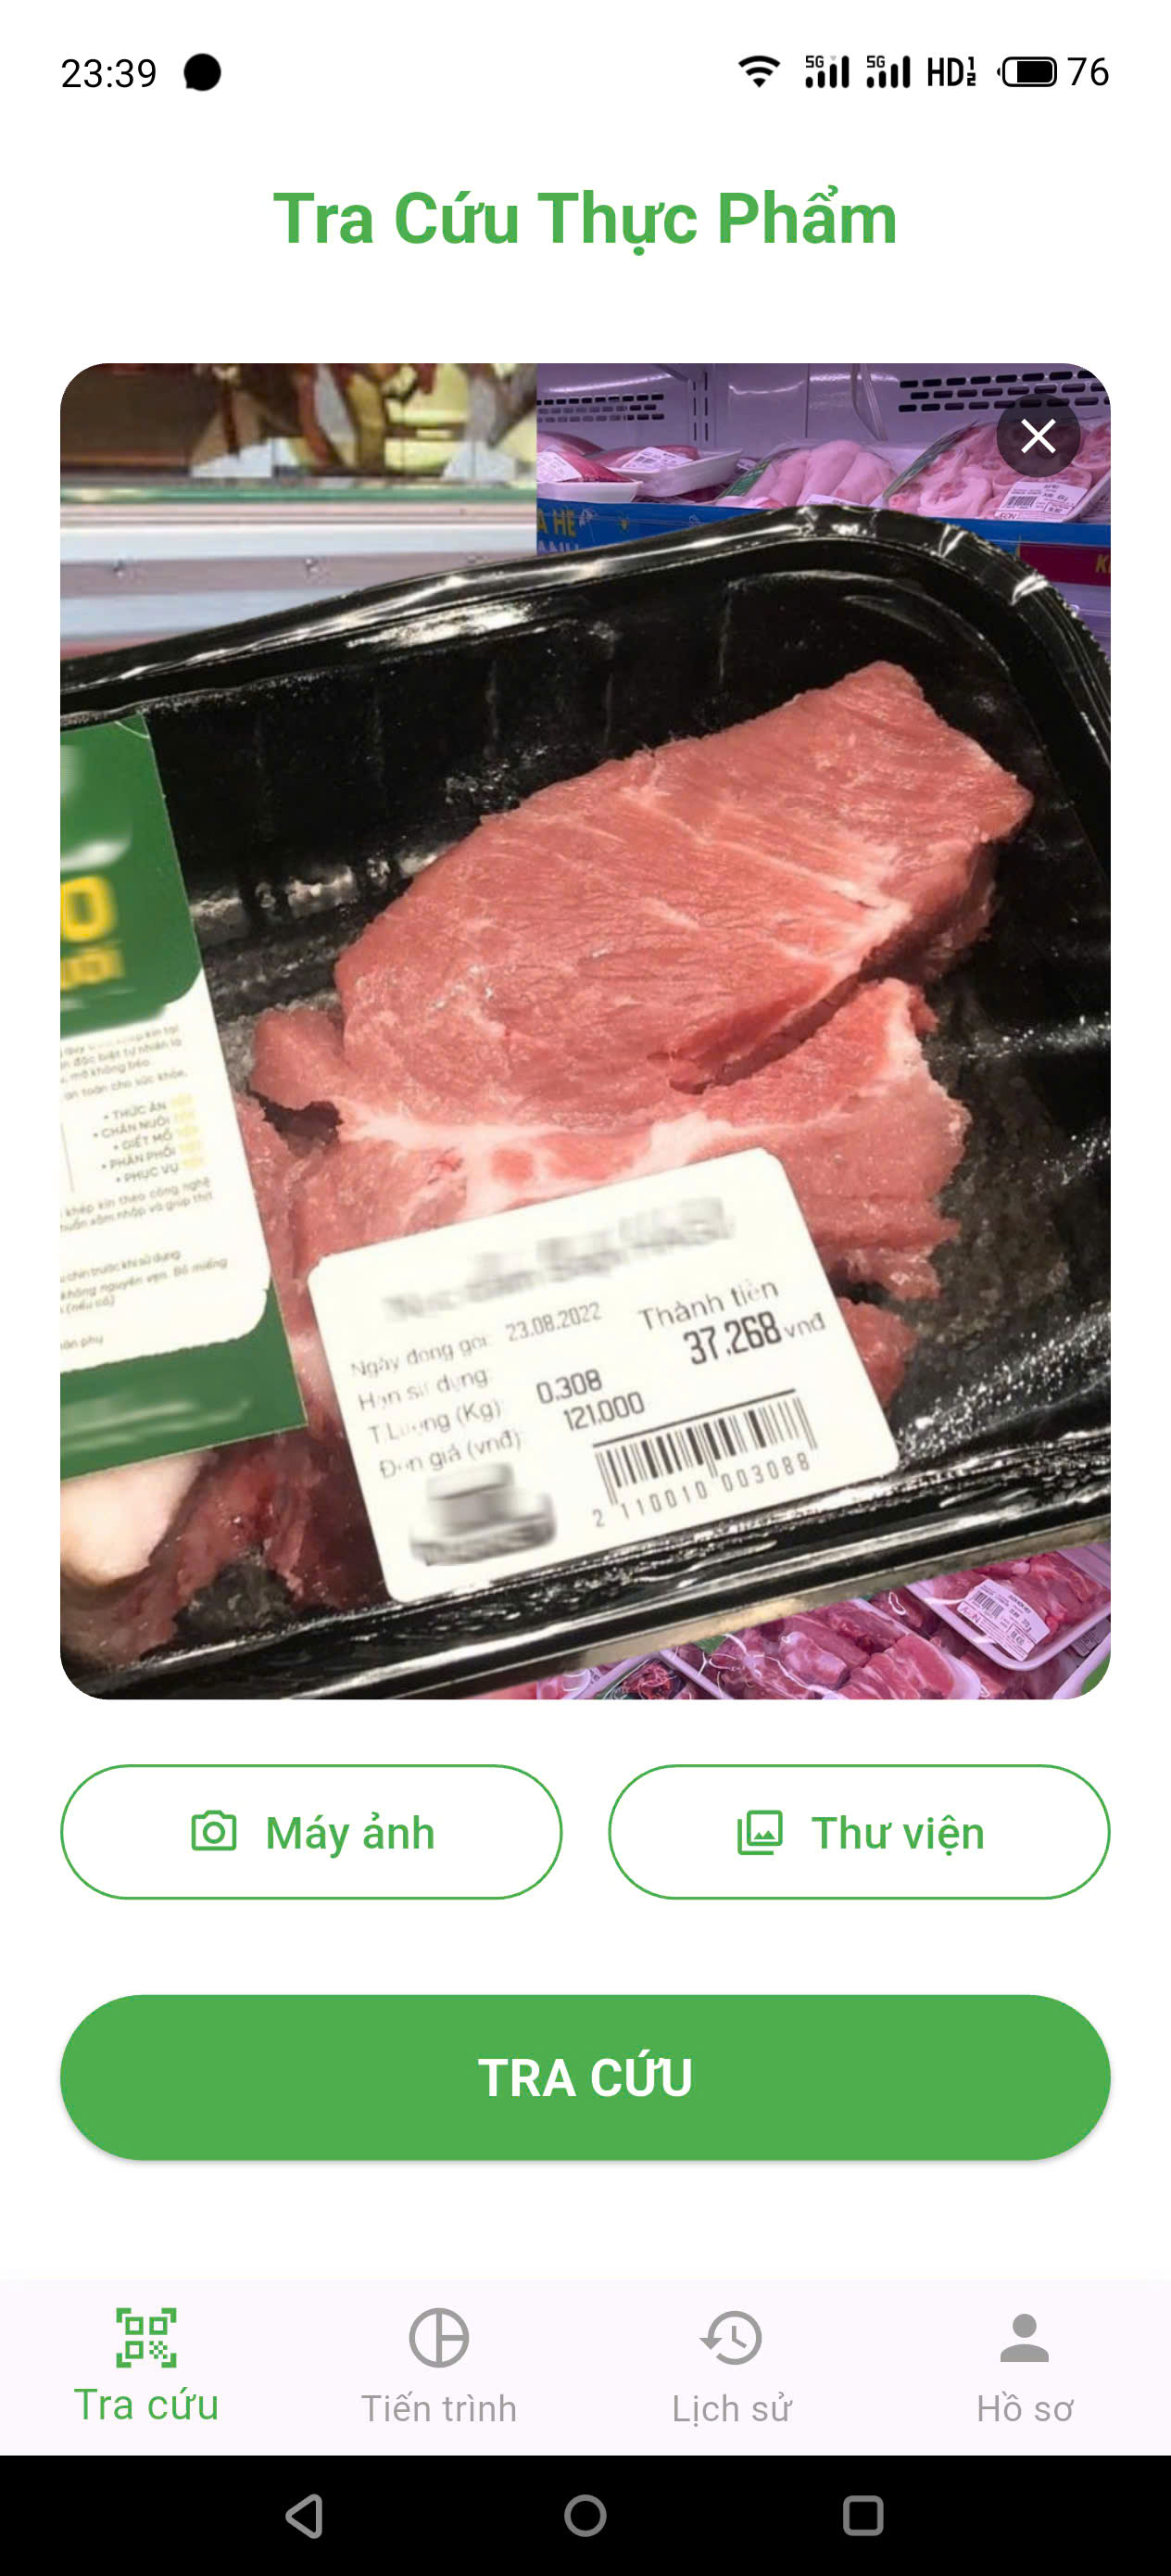
\includegraphics[width=0.88\textwidth,height=0.46\textheight,keepaspectratio]{hinh3_2_man_hinh_quet.jpg}}
        \par\vspace{4pt}{\small (b) Màn hình Quét và Tra cứu}
    \end{minipage}}
    \caption{Giao diện Màn hình Đăng nhập và Màn hình Quét thực phẩm}
    \label{fig:ui_auth_scan}
\end{figure}

Sau khi phân tích ảnh, màn hình kết quả quét (Hình~\ref{fig:ui_found}) gom toàn bộ thao tác vào một luồng trực quan: xem lại ảnh món và tem cân đã cắt (chạm để phóng to), đổi bộ phận cắt hoặc 4 loại trứng, theo dõi số phần chuẩn, chỉnh khối lượng nhãn và chọn tỷ lệ tiêu thụ thực tế $\gamma$, thêm món vào thực đơn hôm nay và xem tư vấn từ chuyên gia AI. Từ đây, người dùng có thể mở bảng đối chiếu chi tiết toàn bộ đa lượng và vi chất theo hai cột $100\text{ g}$ và thực ăn $m_{\text{consumed}}$ (Hình~\ref{fig:ui_result_detail}).

\begin{figure}[htbp]
    \centering
    {\setlength{\fboxsep}{0pt}\setlength{\fboxrule}{0.4pt}%
    \begin{minipage}[b]{0.46\textwidth}
        \centering
        \fcolorbox{black!15}{white}{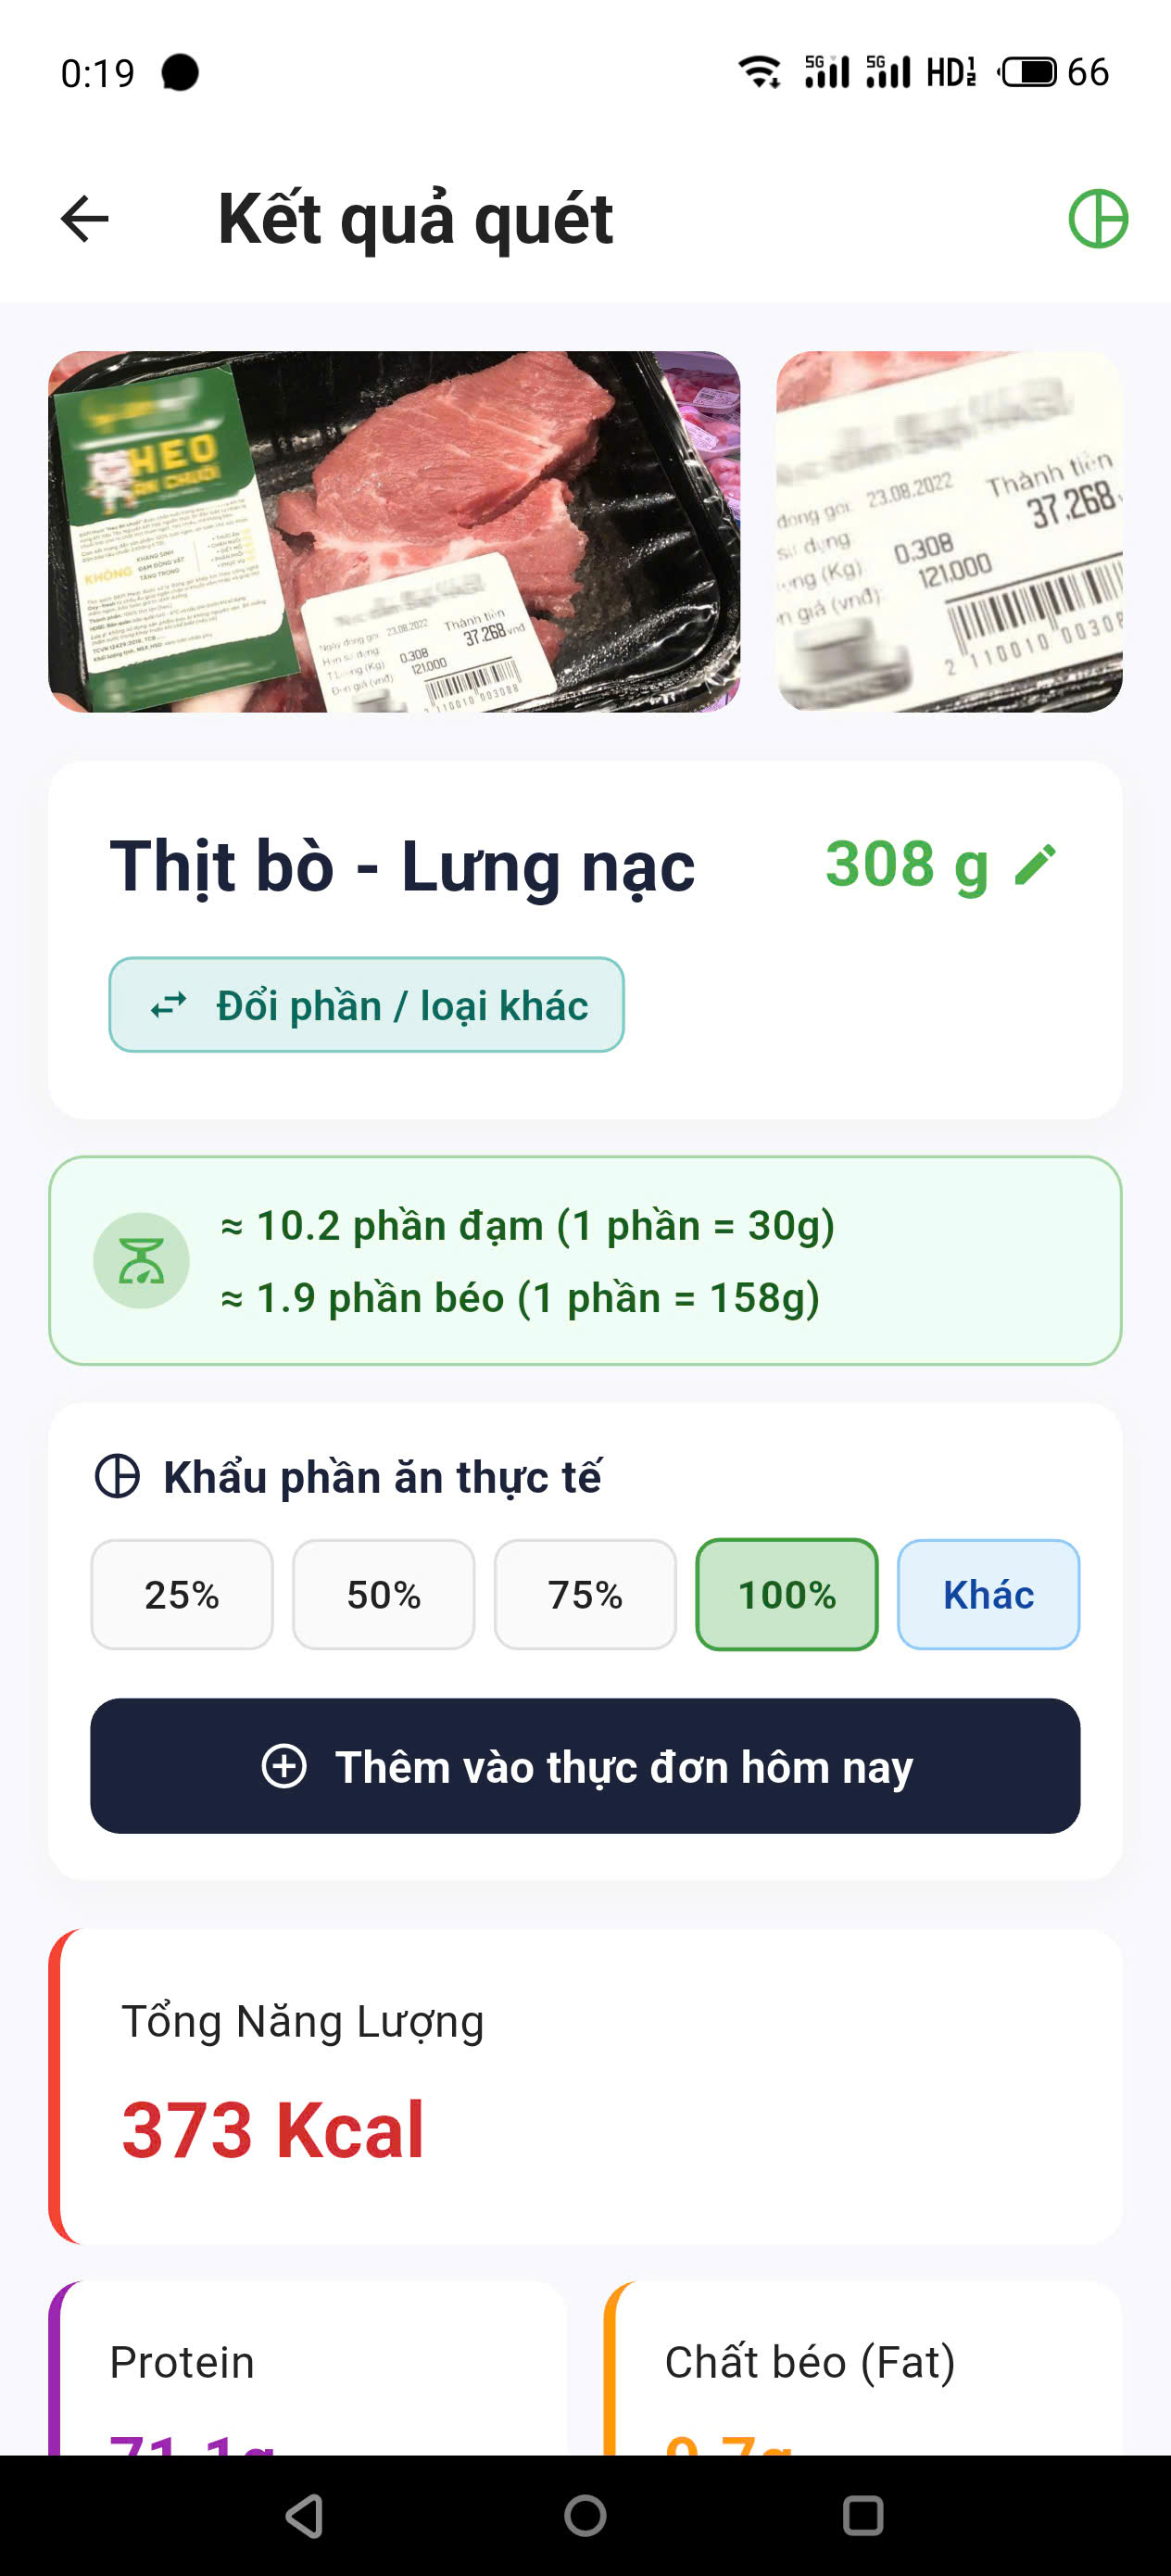
\includegraphics[width=0.88\textwidth,height=0.46\textheight,keepaspectratio]{hinh3_3a_ket_qua_tren.jpg}}
        \par\vspace{4pt}{\small (a) Phần trên: ảnh cắt, phần thịt và tỷ lệ ăn}
    \end{minipage}
    \hfill
    \begin{minipage}[b]{0.46\textwidth}
        \centering
        \fcolorbox{black!15}{white}{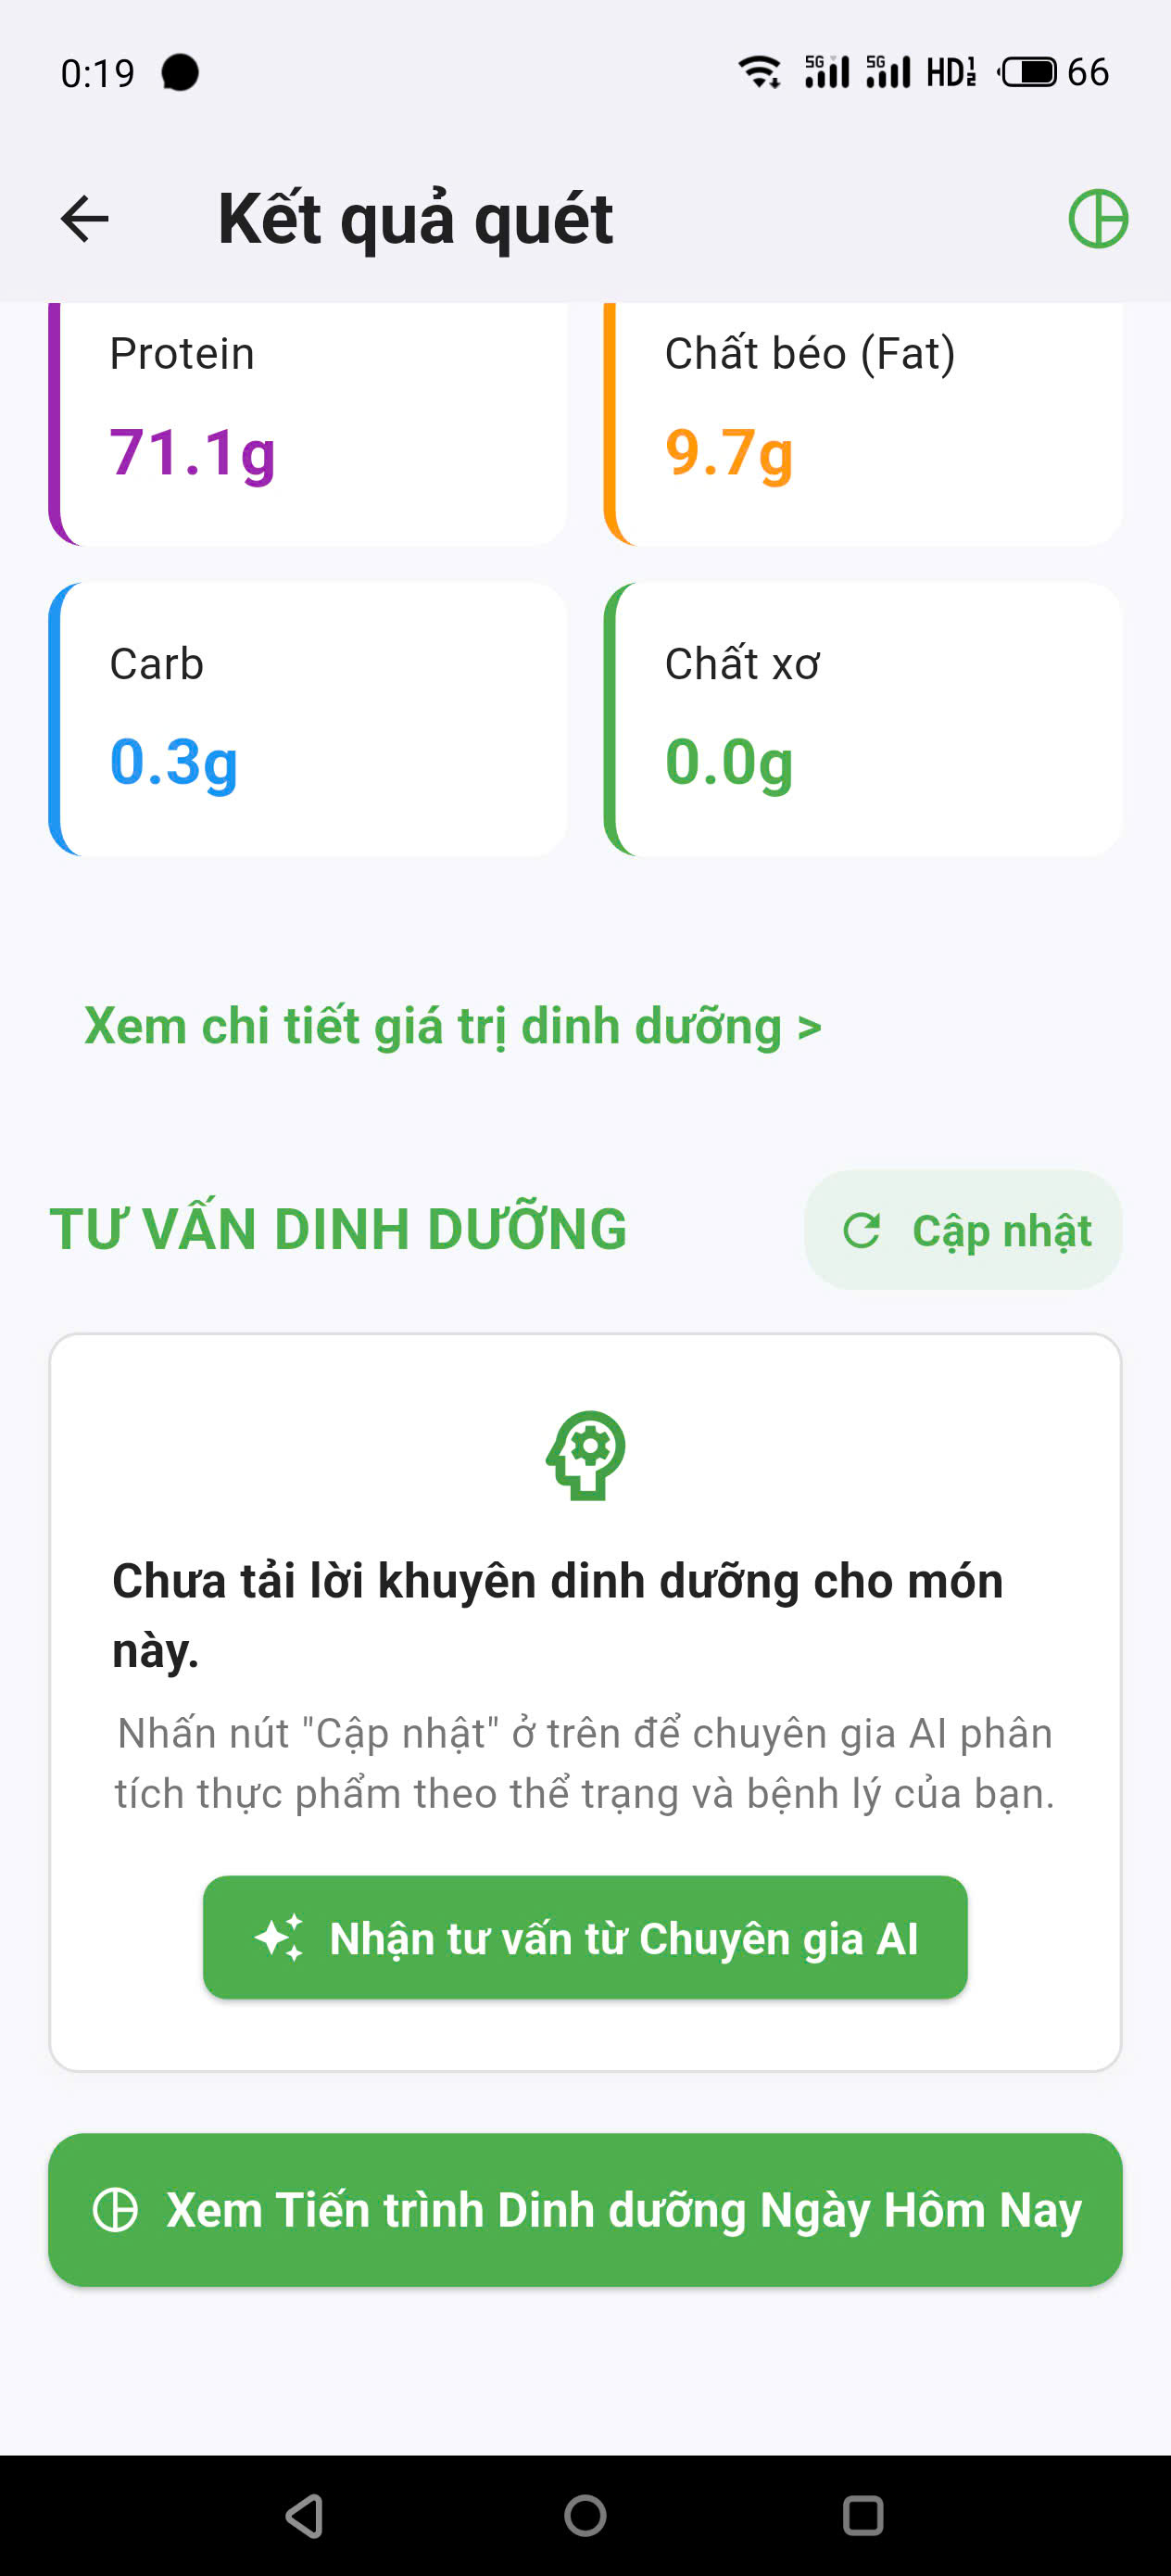
\includegraphics[width=0.88\textwidth,height=0.46\textheight,keepaspectratio]{hinh3_3b_ket_qua_duoi.jpg}}
        \par\vspace{4pt}{\small (b) Phần dưới: đa lượng và tư vấn AI}
    \end{minipage}}
    \caption{Giao diện Màn hình Kết quả Quét trên NutriCare}
    \label{fig:ui_found}
\end{figure}

\begin{figure}[htbp]
    \centering
    {\setlength{\fboxsep}{0pt}\setlength{\fboxrule}{0.4pt}%
    \fcolorbox{black!15}{white}{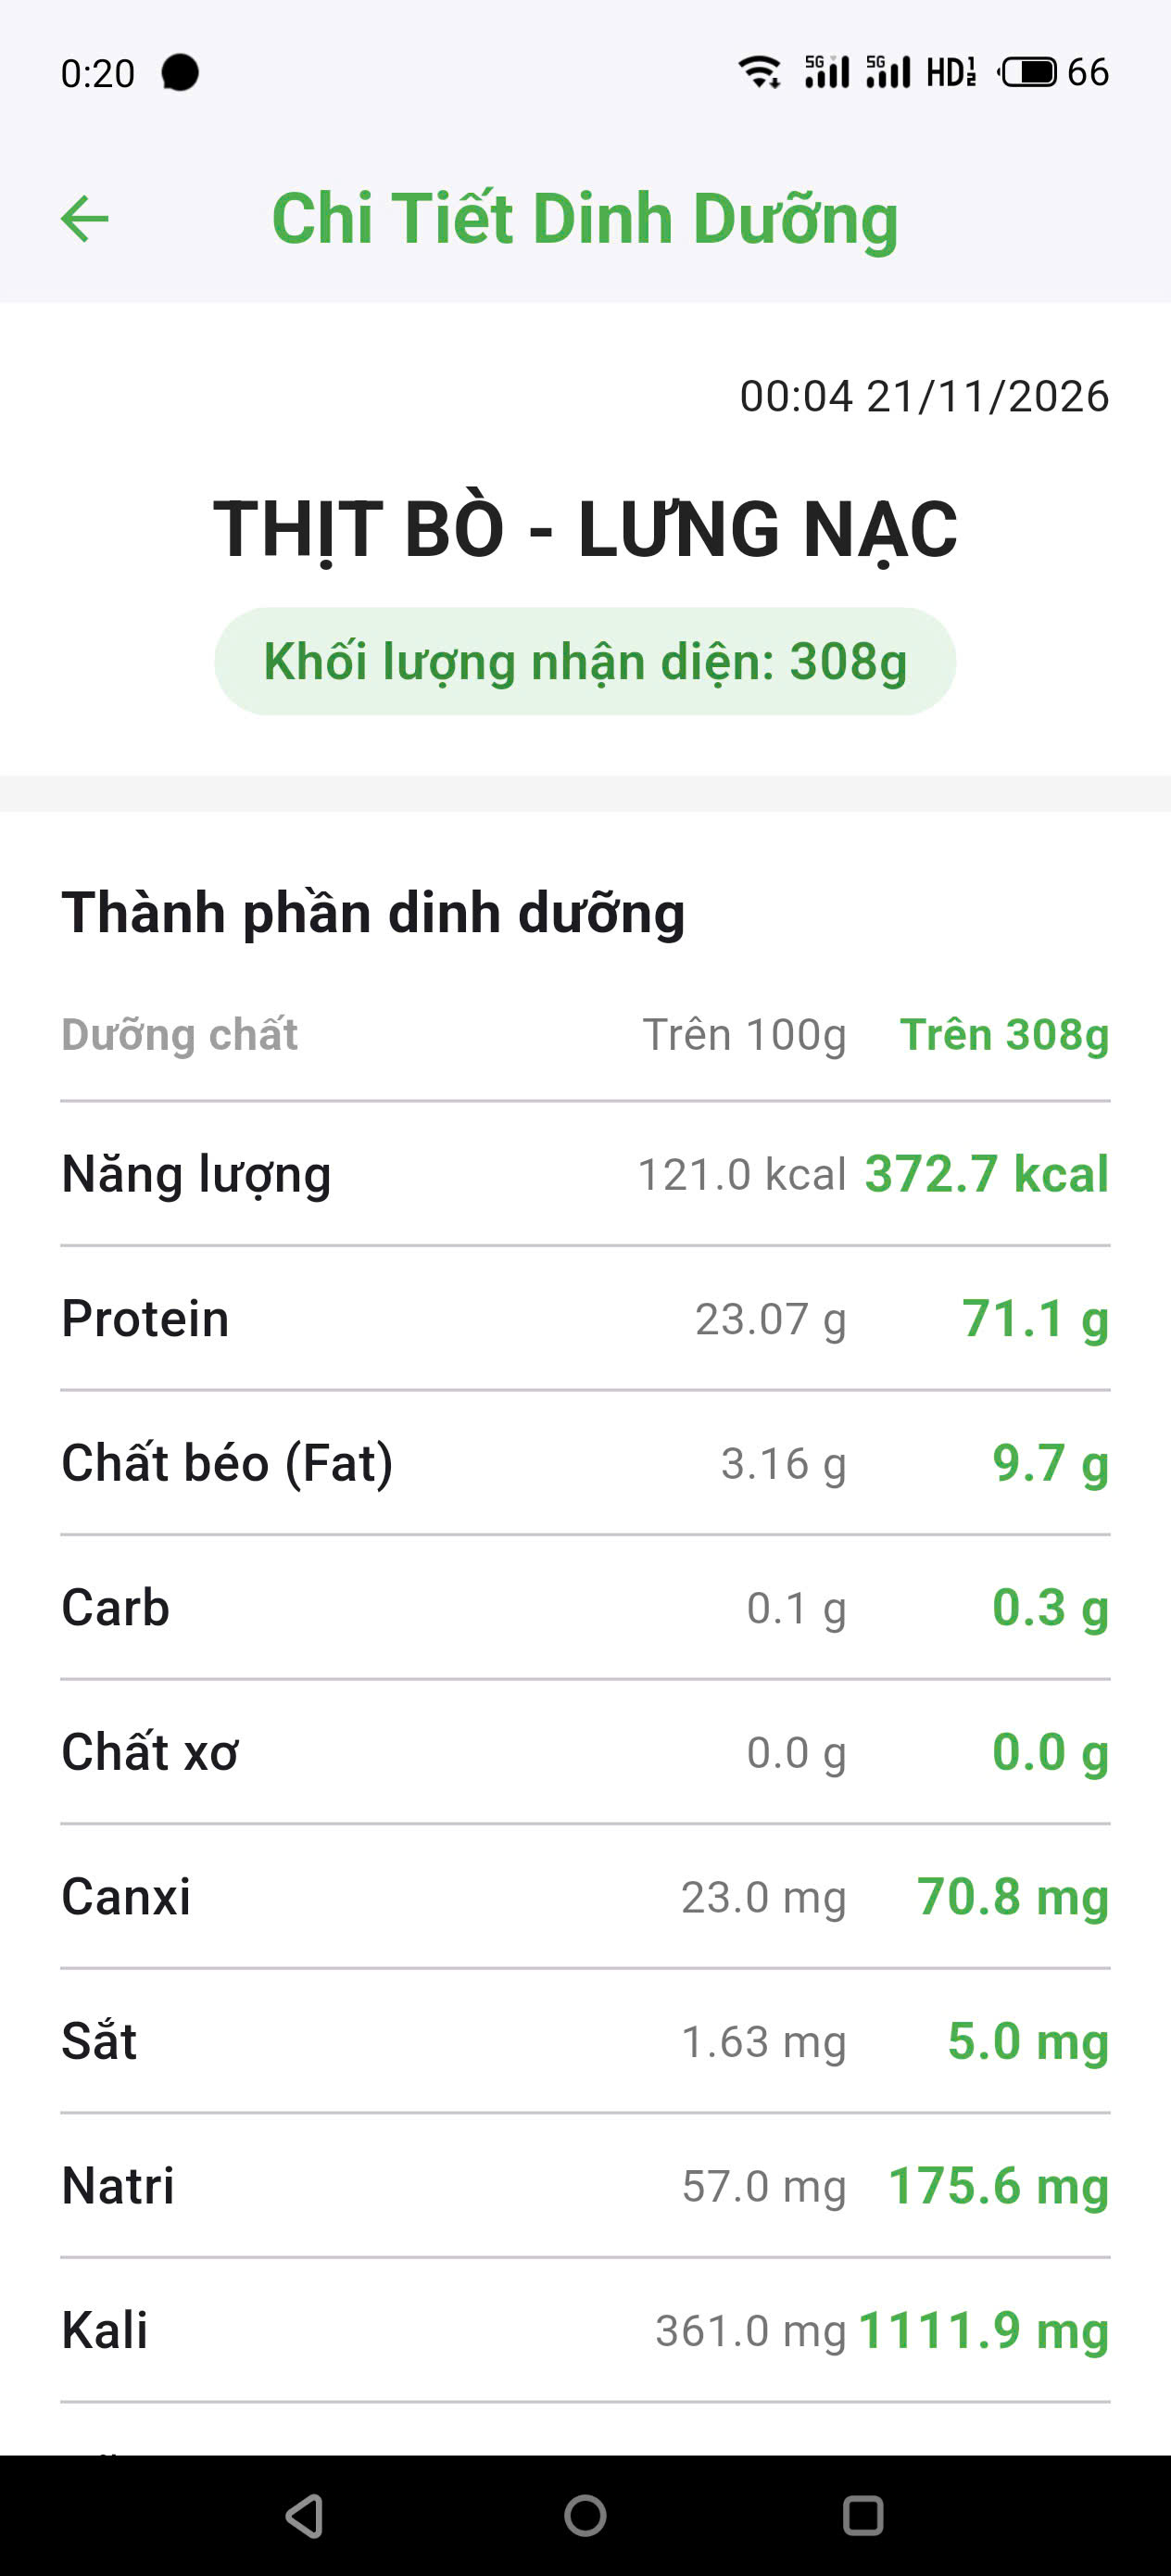
\includegraphics[width=0.42\textwidth,height=0.46\textheight,keepaspectratio]{hinh3_4_chi_tiet_dinh_duong.jpg}}}
    \caption{Bảng Chi tiết Dinh dưỡng đối chiếu mức chuẩn $100\text{ g}$ và khẩu phần thực ăn}
    \label{fig:ui_result_detail}
\end{figure}

Nhóm màn hình theo dõi dài hạn gồm Tiến trình dinh dưỡng ngày (Hình~\ref{fig:ui_progress}) hiển thị lượng calo, các thanh tiến trình đa lượng và 6 ngưỡng vi chất y khoa kèm khối quy đổi phần ăn thiếu hụt (\textit{đạm/tinh bột/béo}), cùng màn hình Lịch sử tra cứu (Hình~\ref{fig:ui_history}) lưu toàn bộ các lần quét có gắn nhãn nhận diện món đã nạp vào thực đơn và hỗ trợ chọn nhiều mục để xóa.

\begin{figure}[htbp]
    \centering
    {\setlength{\fboxsep}{0pt}\setlength{\fboxrule}{0.4pt}%
    \begin{minipage}[b]{0.46\textwidth}
        \centering
        \fcolorbox{black!15}{white}{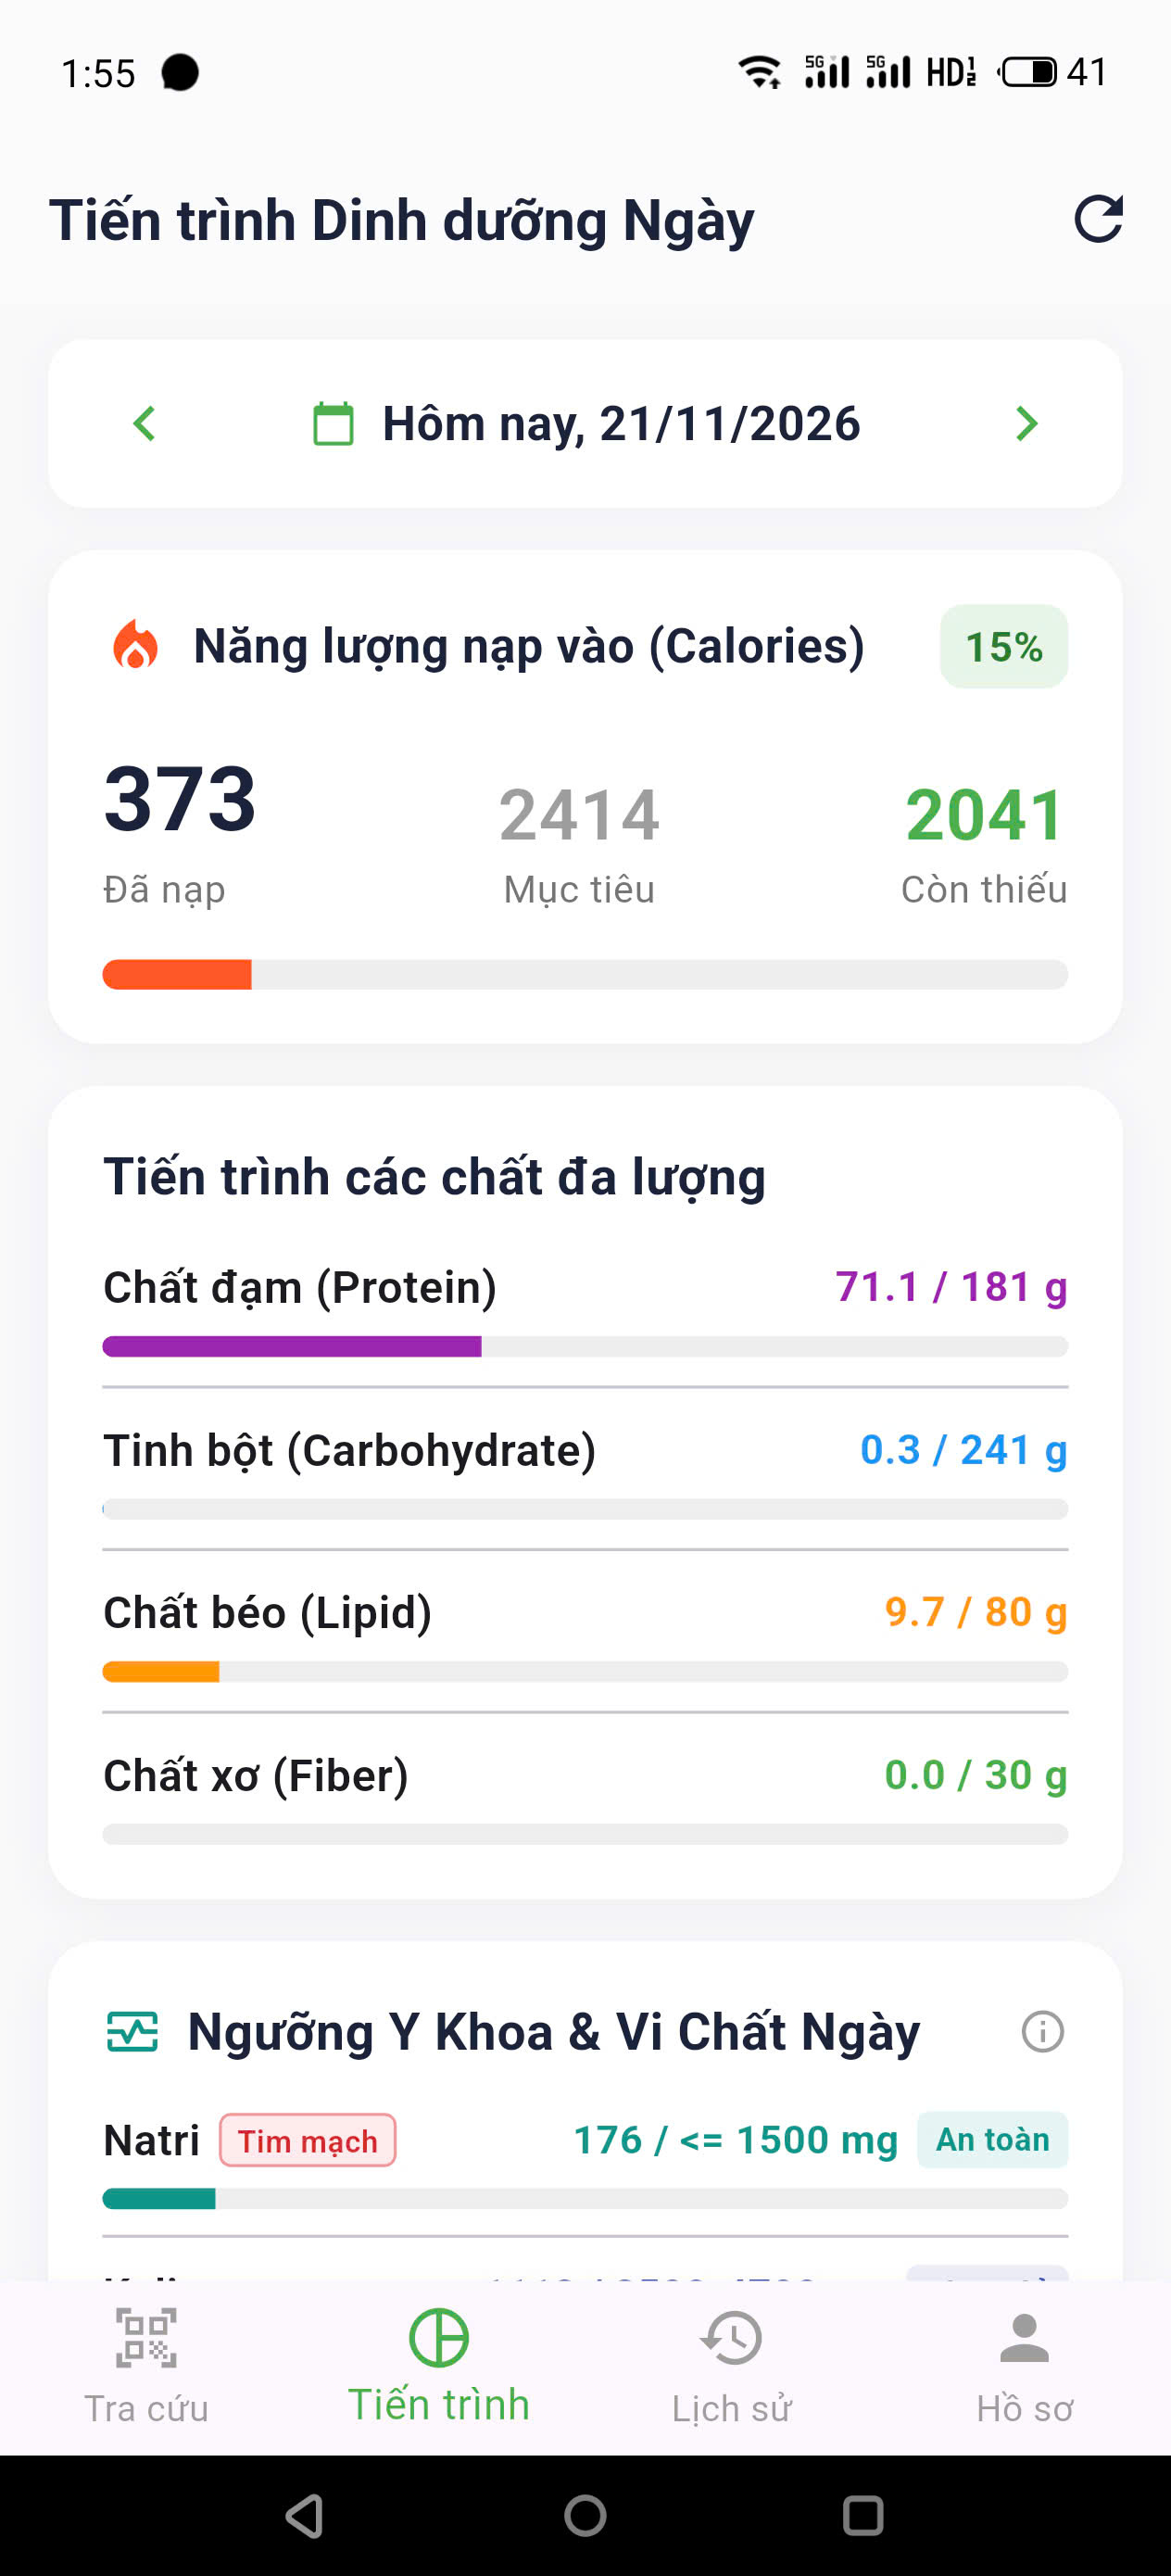
\includegraphics[width=0.88\textwidth,height=0.46\textheight,keepaspectratio]{hinh3_5a_tien_trinh_tren.jpg}}
        \par\vspace{4pt}{\small (a) Phần trên: calo và các chất đa lượng}
    \end{minipage}
    \hfill
    \begin{minipage}[b]{0.46\textwidth}
        \centering
        \fcolorbox{black!15}{white}{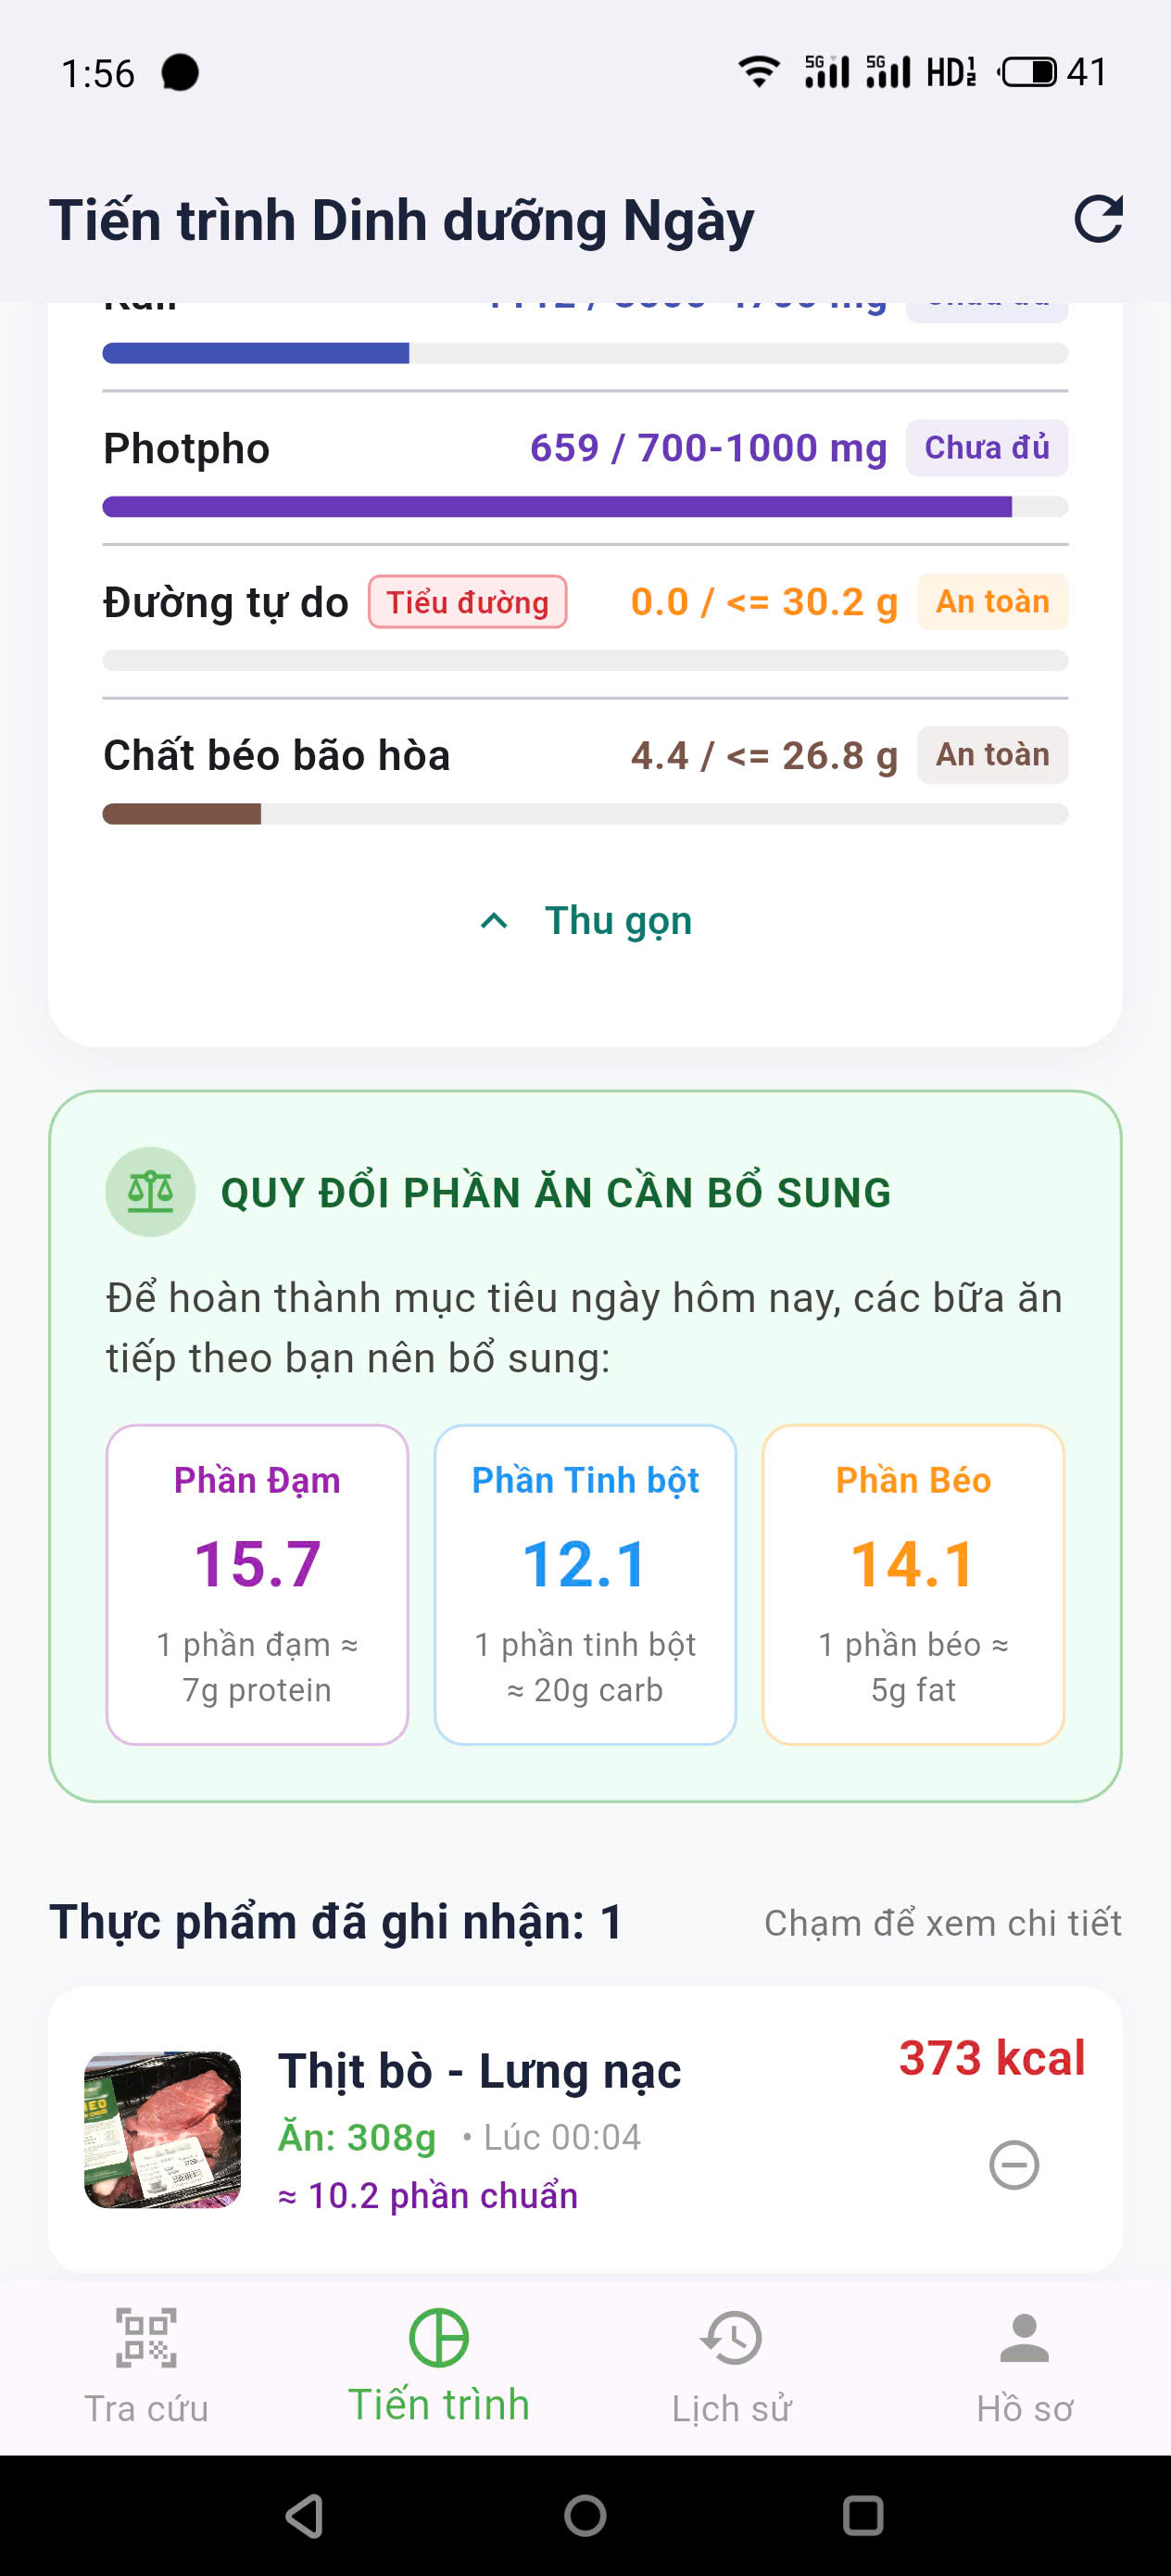
\includegraphics[width=0.88\textwidth,height=0.46\textheight,keepaspectratio]{hinh3_5b_tien_trinh_duoi.jpg}}
        \par\vspace{4pt}{\small (b) Phần dưới: ngưỡng y khoa và quy đổi phần ăn}
    \end{minipage}}
    \caption{Giao diện Màn hình Tiến trình Dinh dưỡng Ngày}
    \label{fig:ui_progress}
\end{figure}

\begin{figure}[htbp]
    \centering
    {\setlength{\fboxsep}{0pt}\setlength{\fboxrule}{0.4pt}%
    \fcolorbox{black!15}{white}{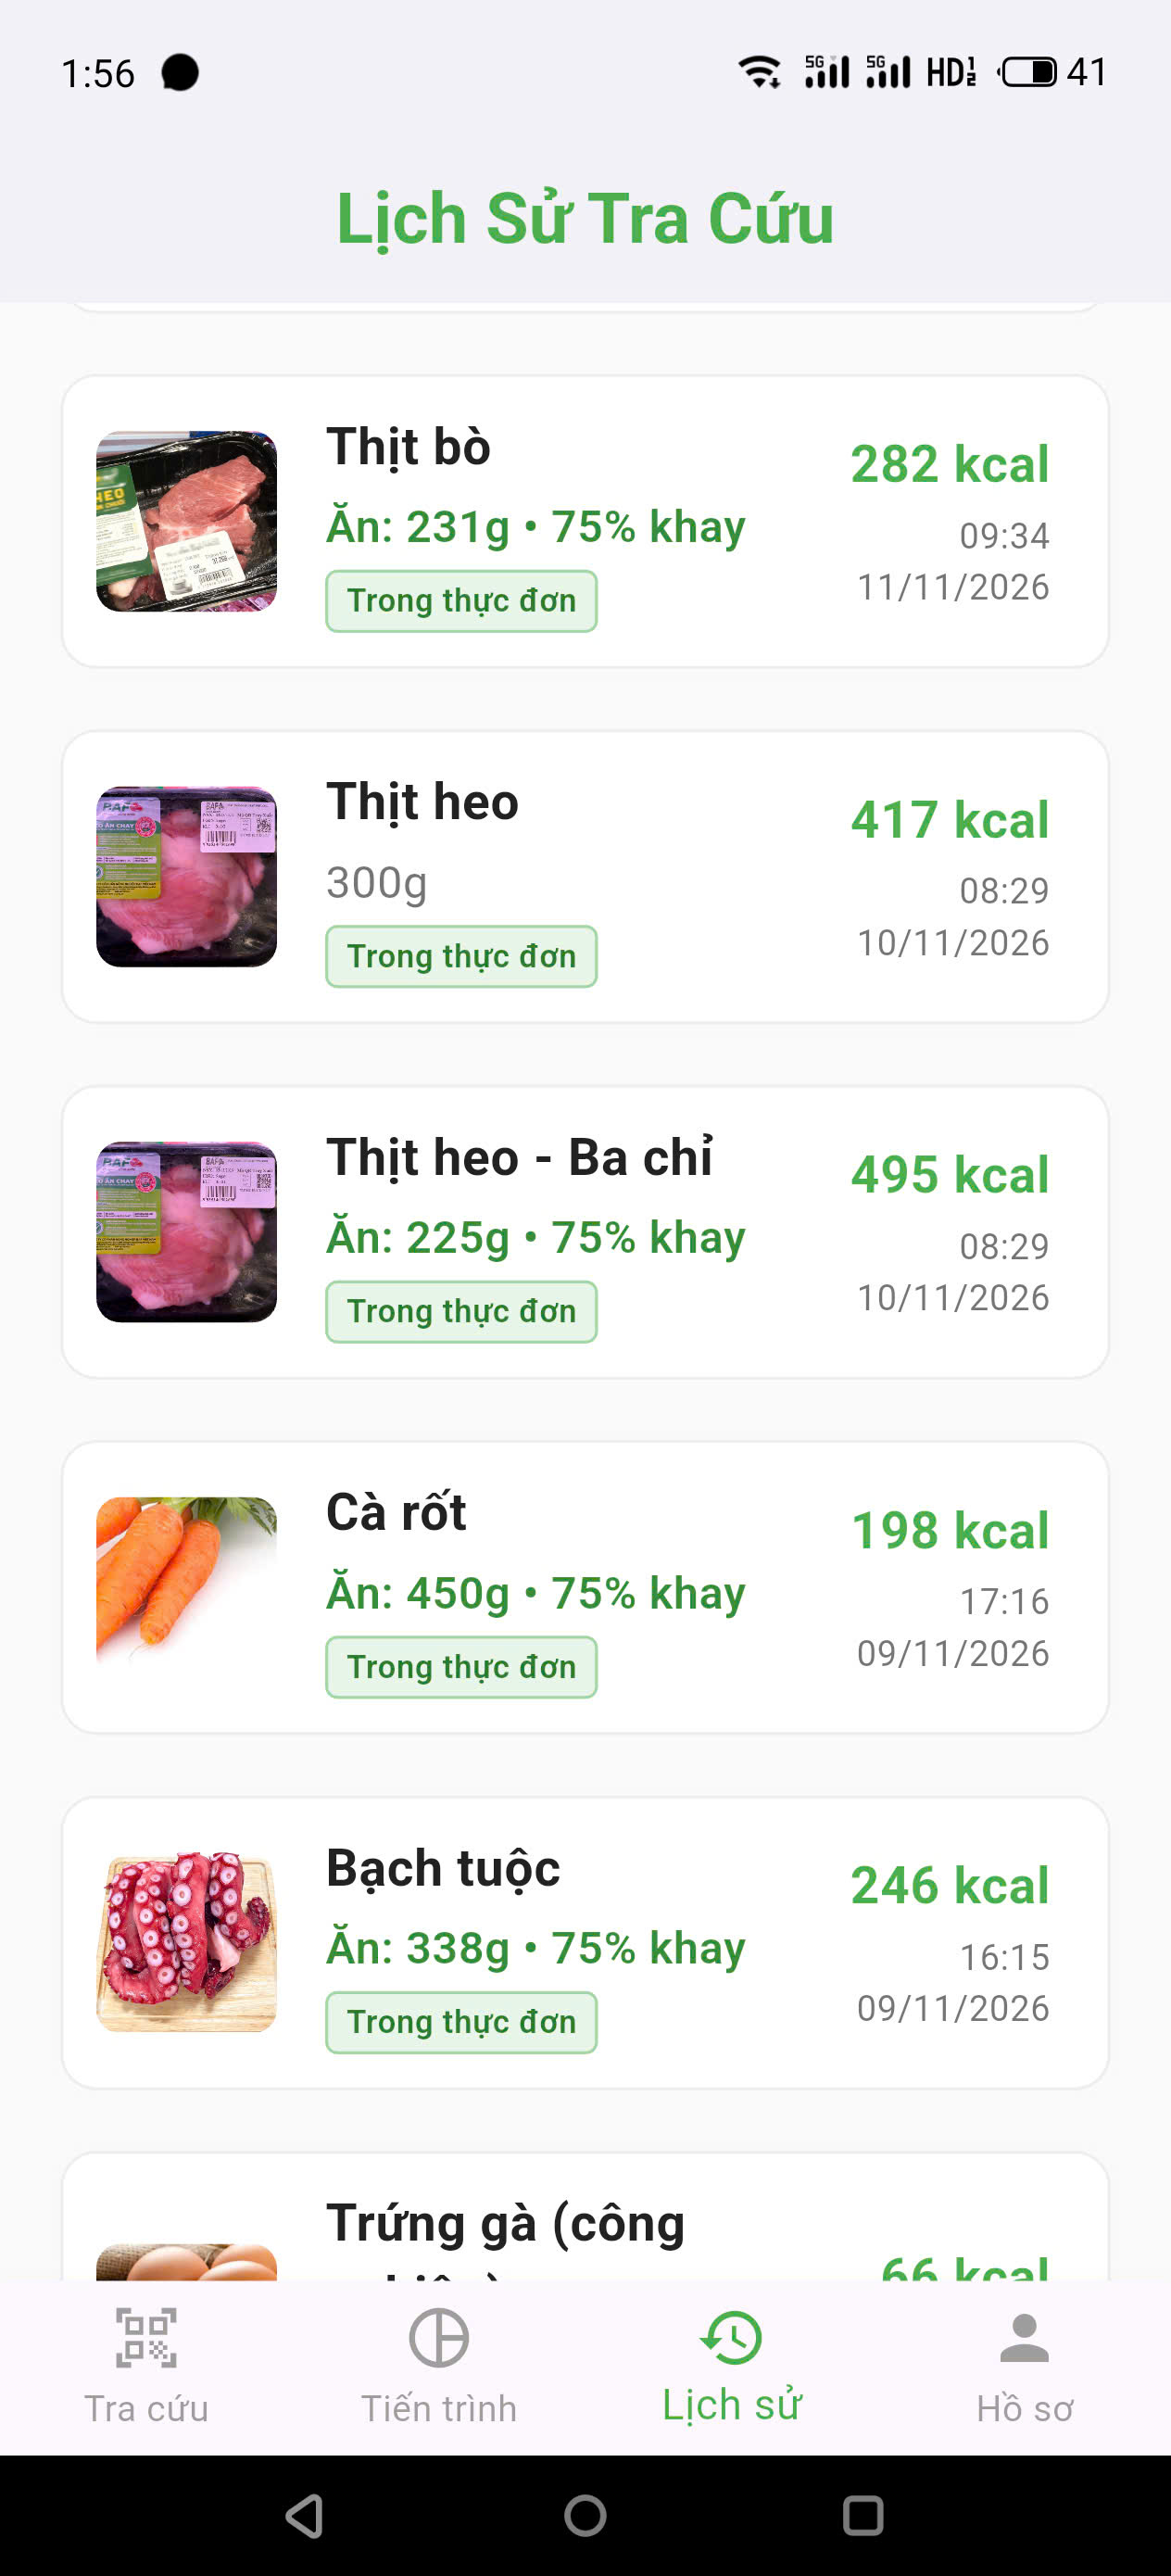
\includegraphics[width=0.42\textwidth,height=0.46\textheight,keepaspectratio]{hinh3_6_lich_su_tra_cuu.jpg}}}
    \caption{Giao diện Màn hình Lịch sử Tra cứu thực phẩm}
    \label{fig:ui_history}
\end{figure}

Màn hình Hồ sơ cá nhân (Hình~\ref{fig:ui_profile}) trình bày tài khoản Google, chỉ số cơ thể kèm các khung giải thích công thức xổ xuống, công tắc kiểm soát béo phì và danh mục giới hạn y khoa; biểu tượng chỉnh sửa đưa tới màn hình Thiết lập hồ sơ (Hình~\ref{fig:ui_edit_profile}) hỗ trợ cảnh báo xung đột mục tiêu theo $\mathrm{BMI}$ và chọn dị ứng/bệnh lý. Ở chế độ Khách, các màn hình yêu cầu tài khoản hiển thị thông báo khóa kèm nút đăng nhập Google ngay tại chỗ để hợp nhất dữ liệu tức thì (Hình~\ref{fig:ui_guest_locked}).

\begin{figure}[htbp]
    \centering
    {\setlength{\fboxsep}{0pt}\setlength{\fboxrule}{0.4pt}%
    \begin{minipage}[b]{0.46\textwidth}
        \centering
        \fcolorbox{black!15}{white}{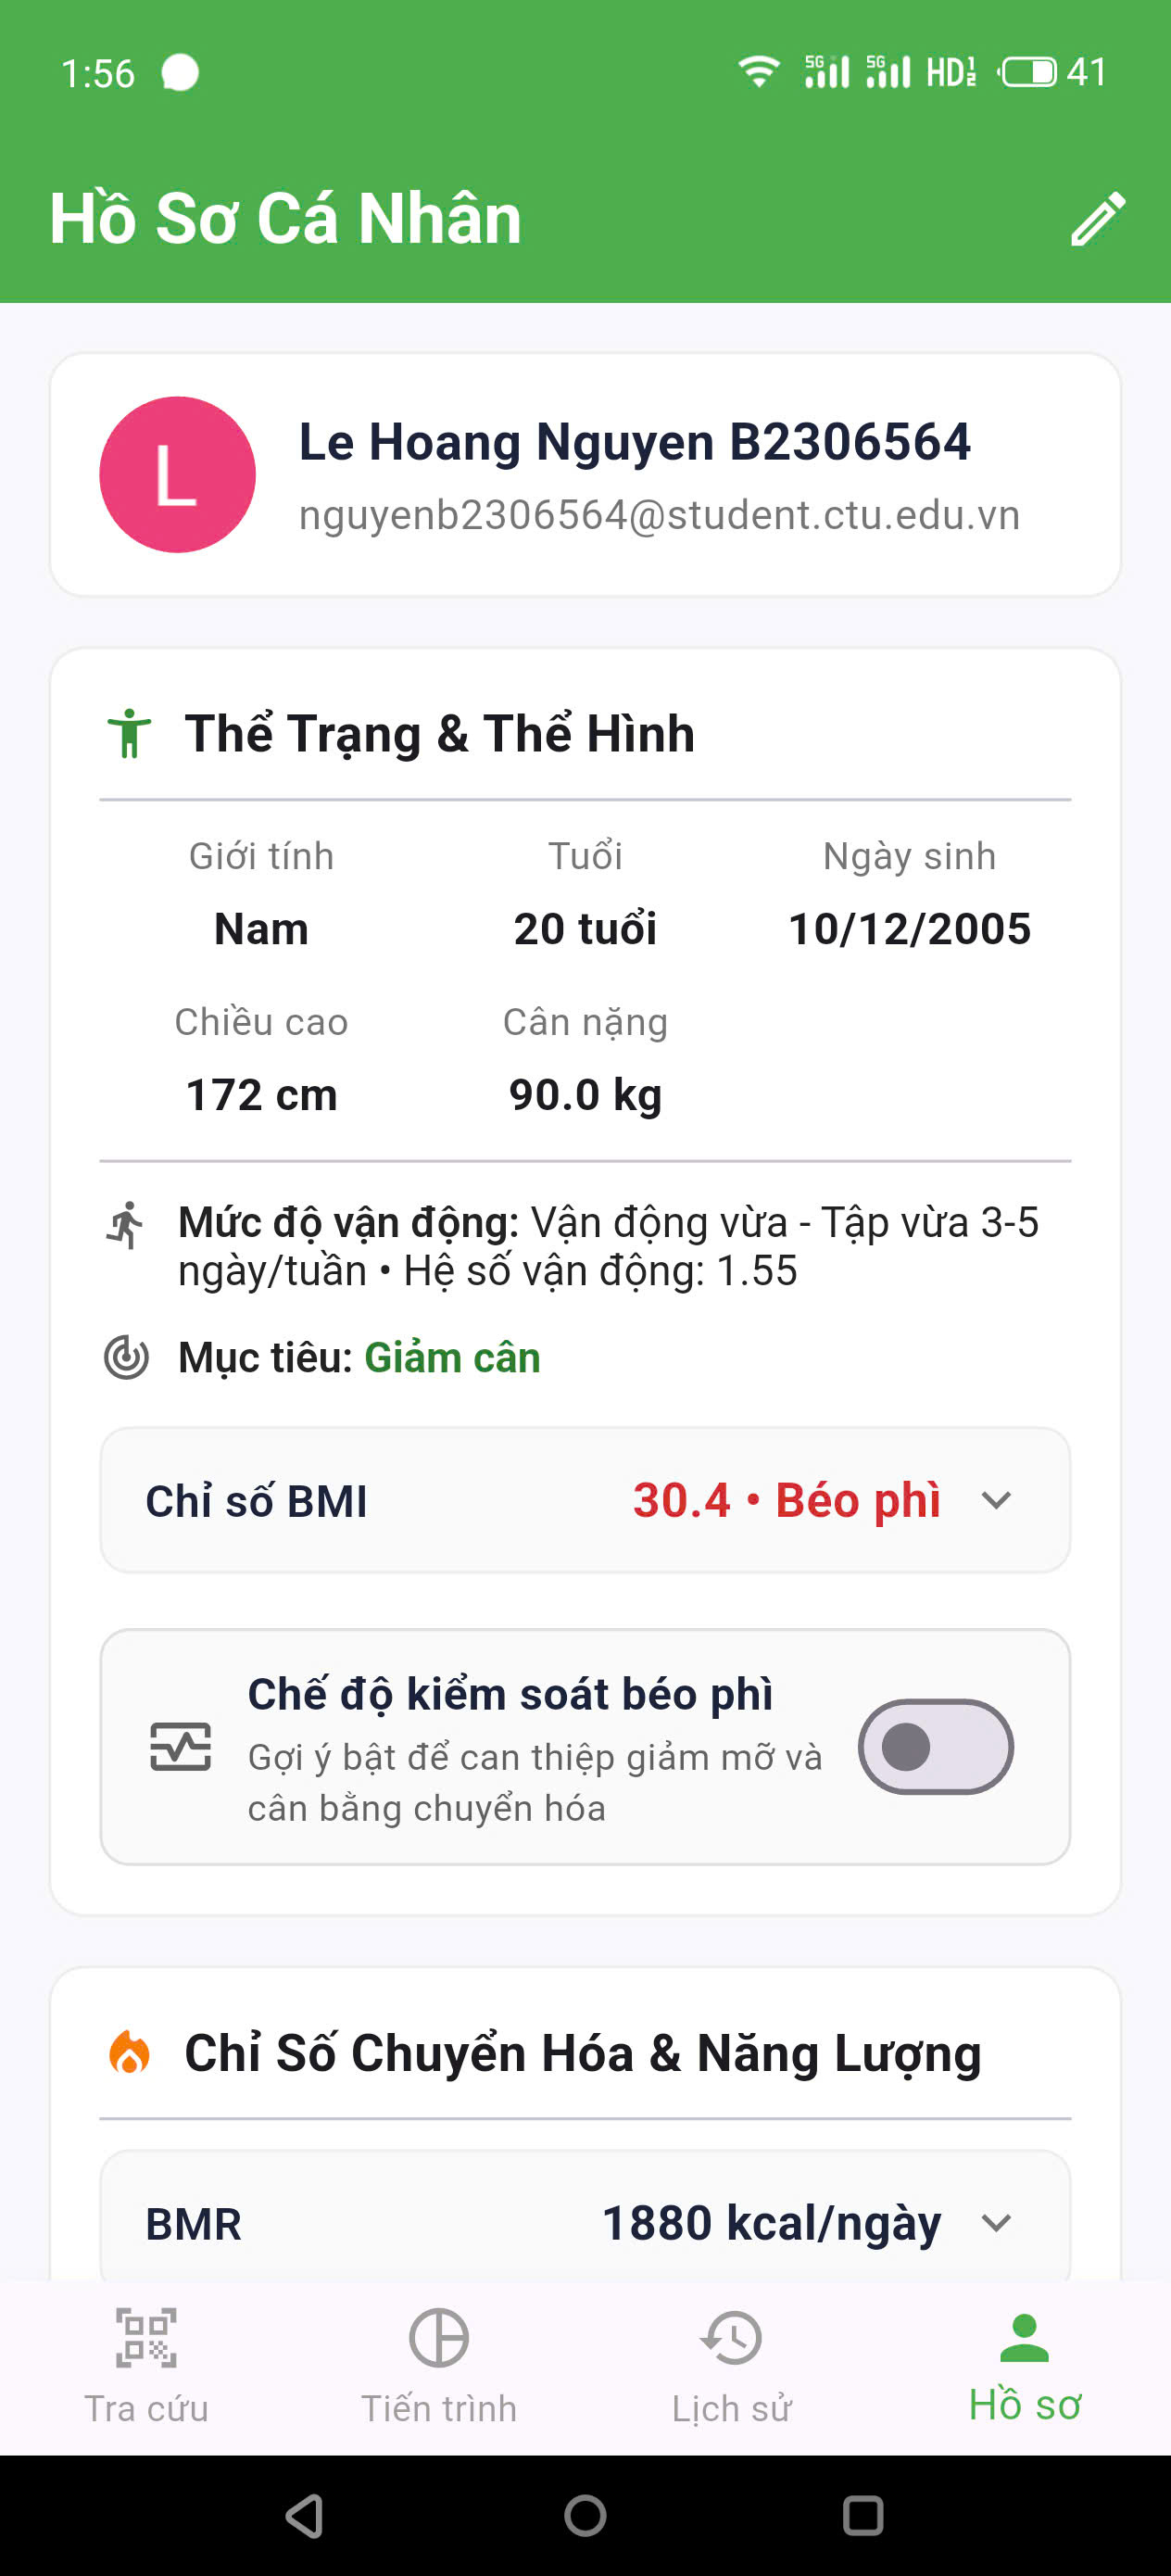
\includegraphics[width=0.88\textwidth,height=0.46\textheight,keepaspectratio]{hinh3_7a_ho_so_tren.jpg}}
        \par\vspace{4pt}{\small (a) Phần trên: tài khoản, thể trạng và BMI}
    \end{minipage}
    \hfill
    \begin{minipage}[b]{0.46\textwidth}
        \centering
        \fcolorbox{black!15}{white}{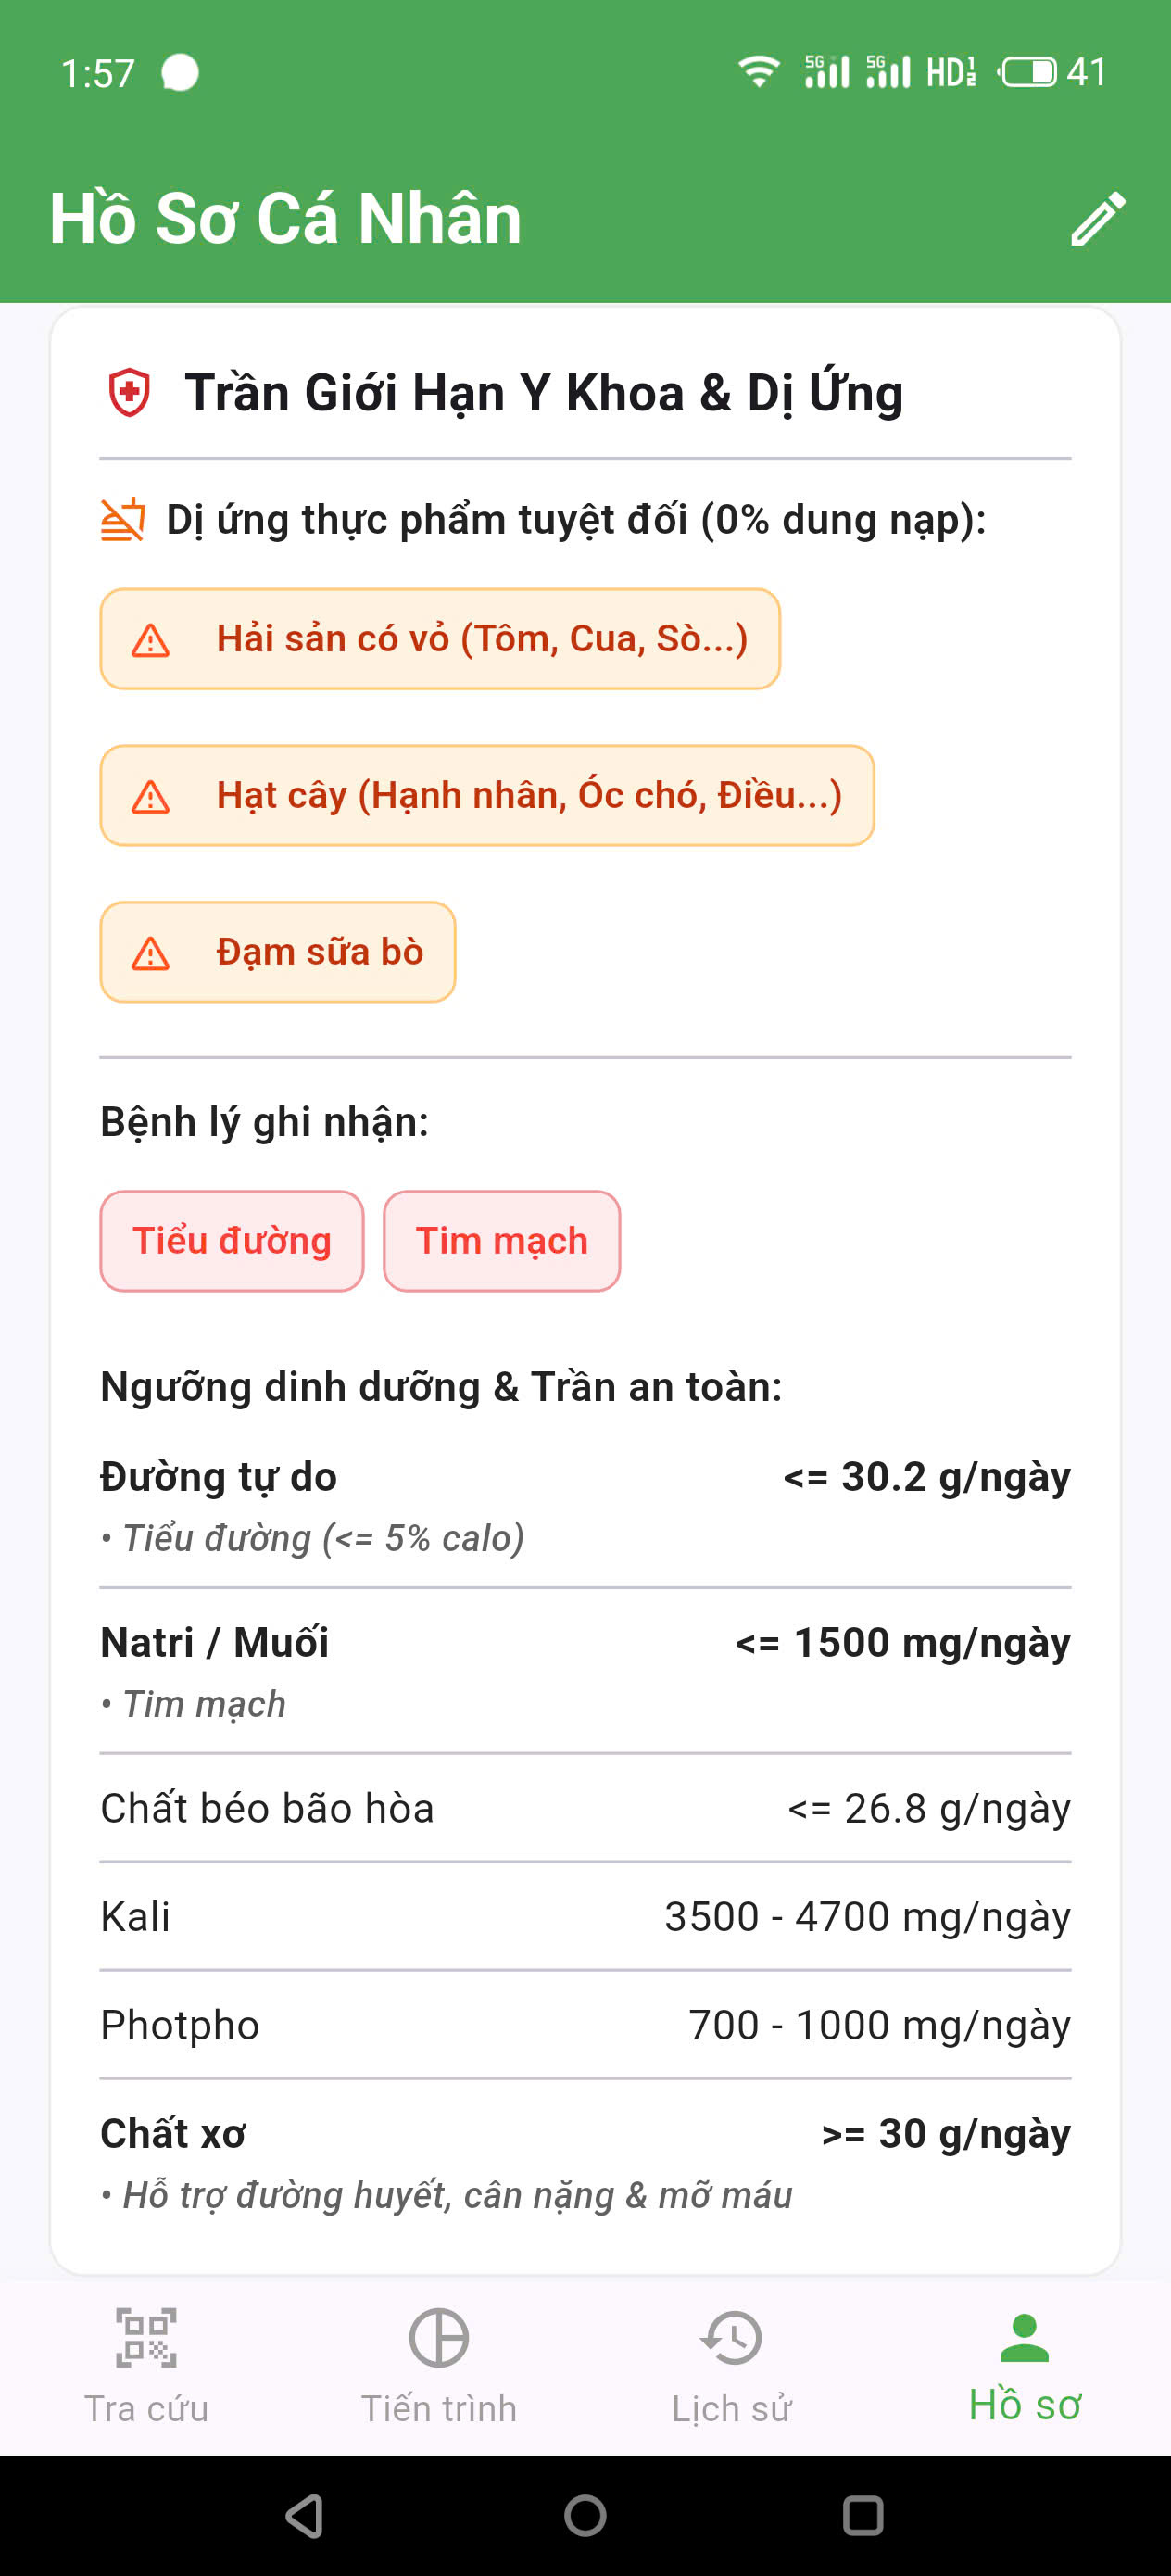
\includegraphics[width=0.88\textwidth,height=0.46\textheight,keepaspectratio]{hinh3_7b_ho_so_duoi.jpg}}
        \par\vspace{4pt}{\small (b) Phần dưới: dị ứng, bệnh lý và trần an toàn}
    \end{minipage}}
    \caption{Giao diện Màn hình Hồ sơ Cá nhân}
    \label{fig:ui_profile}
\end{figure}

\begin{figure}[htbp]
    \centering
    {\setlength{\fboxsep}{0pt}\setlength{\fboxrule}{0.4pt}%
    \begin{minipage}[b]{0.46\textwidth}
        \centering
        \fcolorbox{black!15}{white}{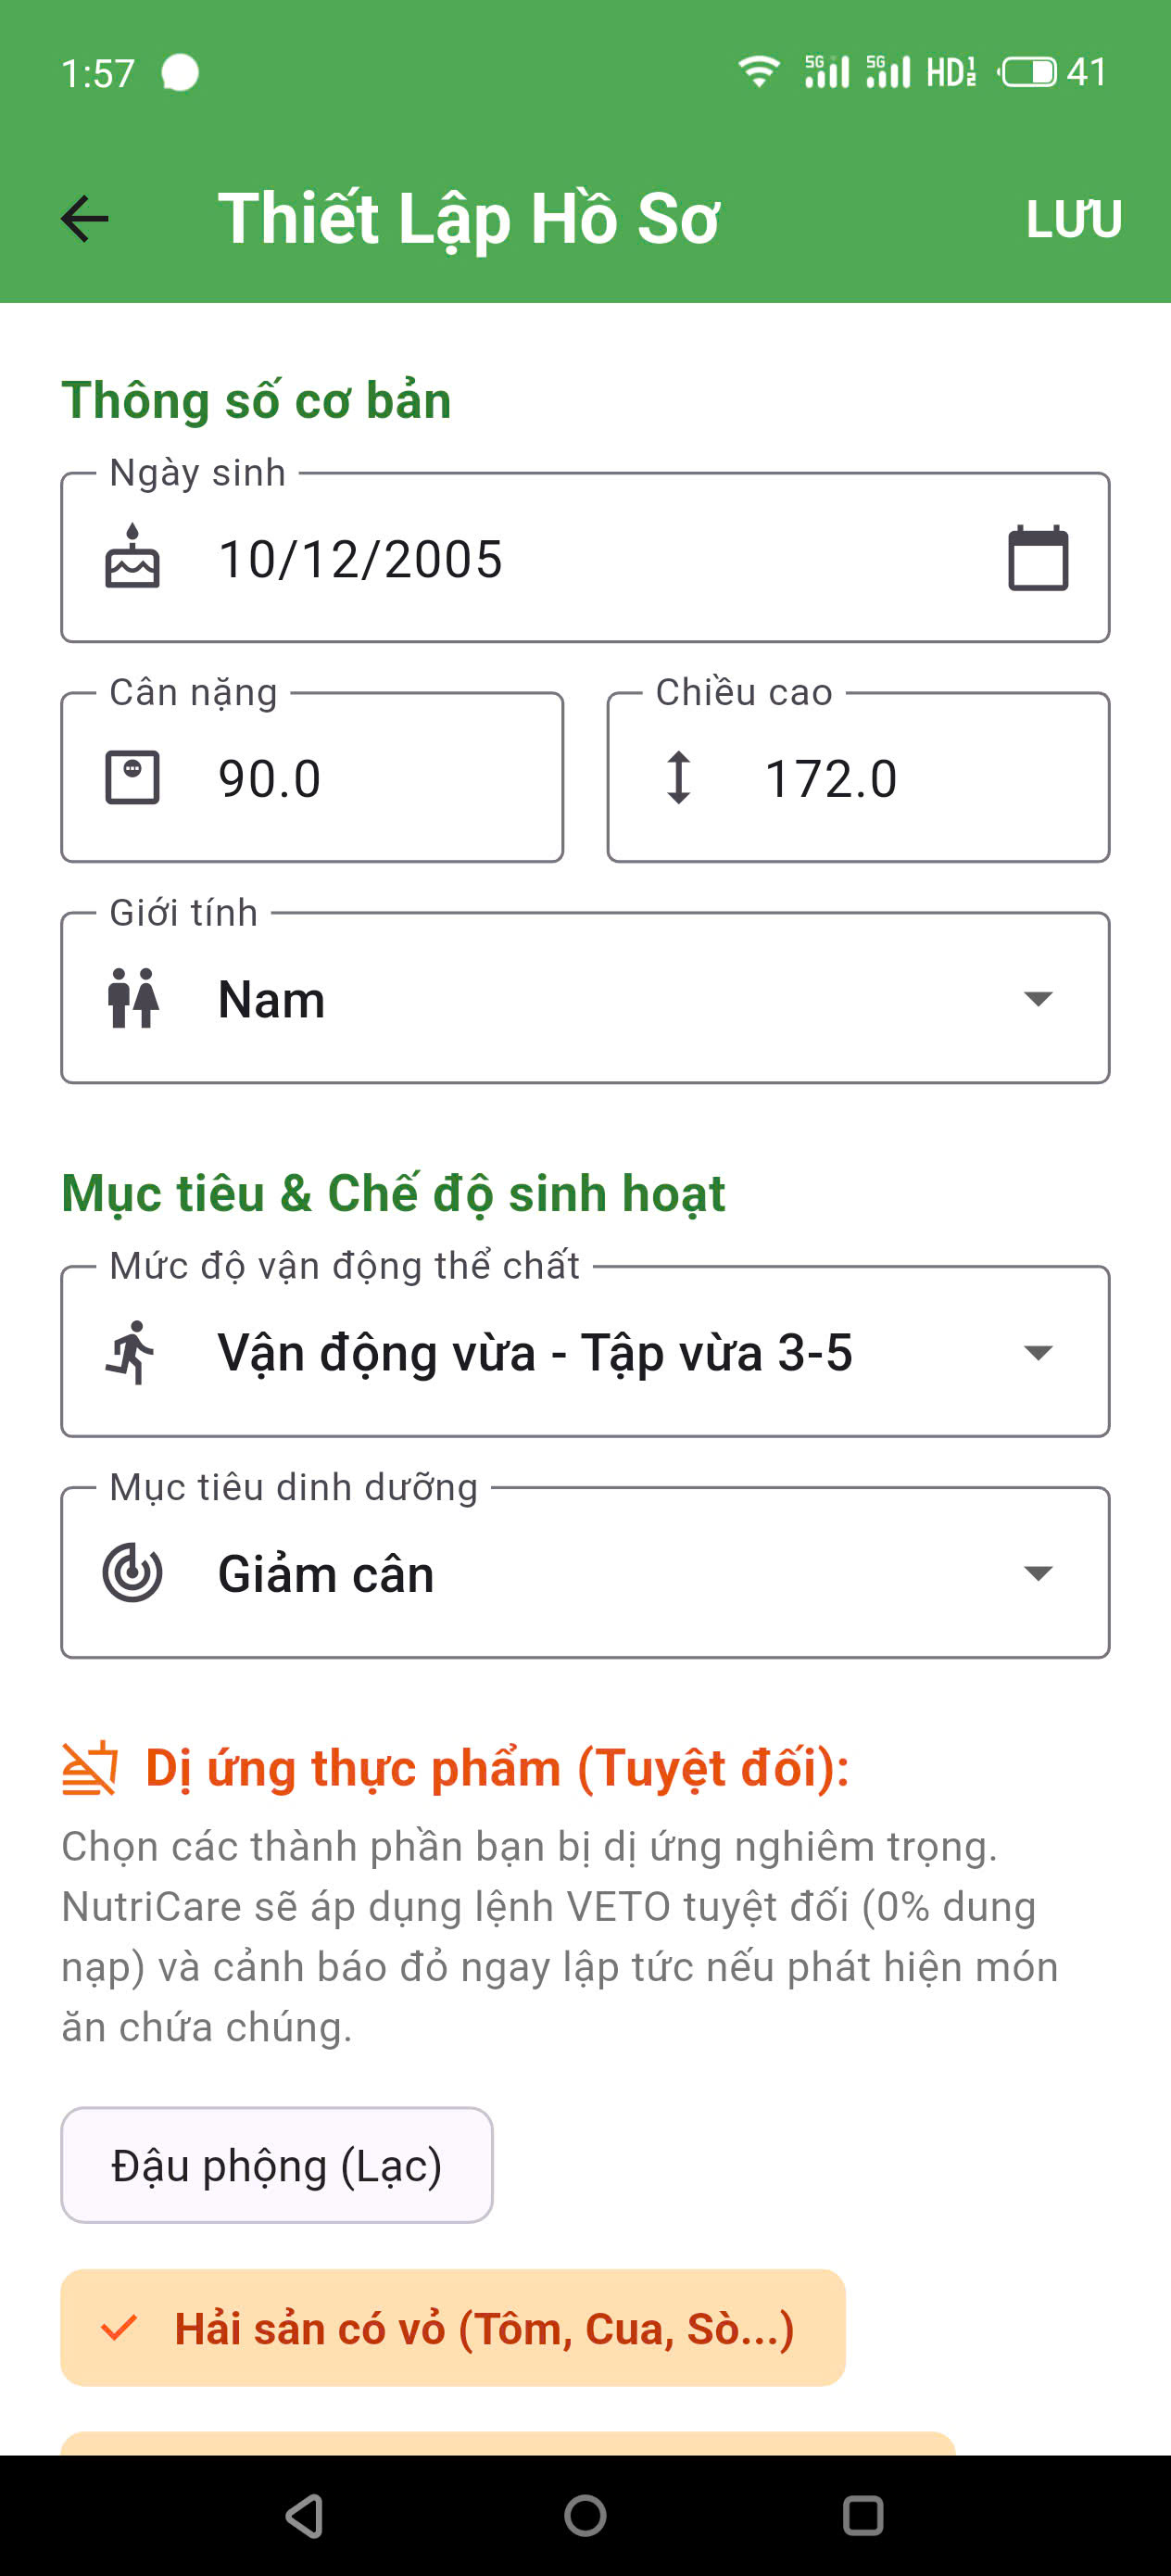
\includegraphics[width=0.88\textwidth,height=0.46\textheight,keepaspectratio]{hinh3_8a_thiet_lap_tren.jpg}}
        \par\vspace{4pt}{\small (a) Phần trên: thông số cơ thể và mục tiêu}
    \end{minipage}
    \hfill
    \begin{minipage}[b]{0.46\textwidth}
        \centering
        \fcolorbox{black!15}{white}{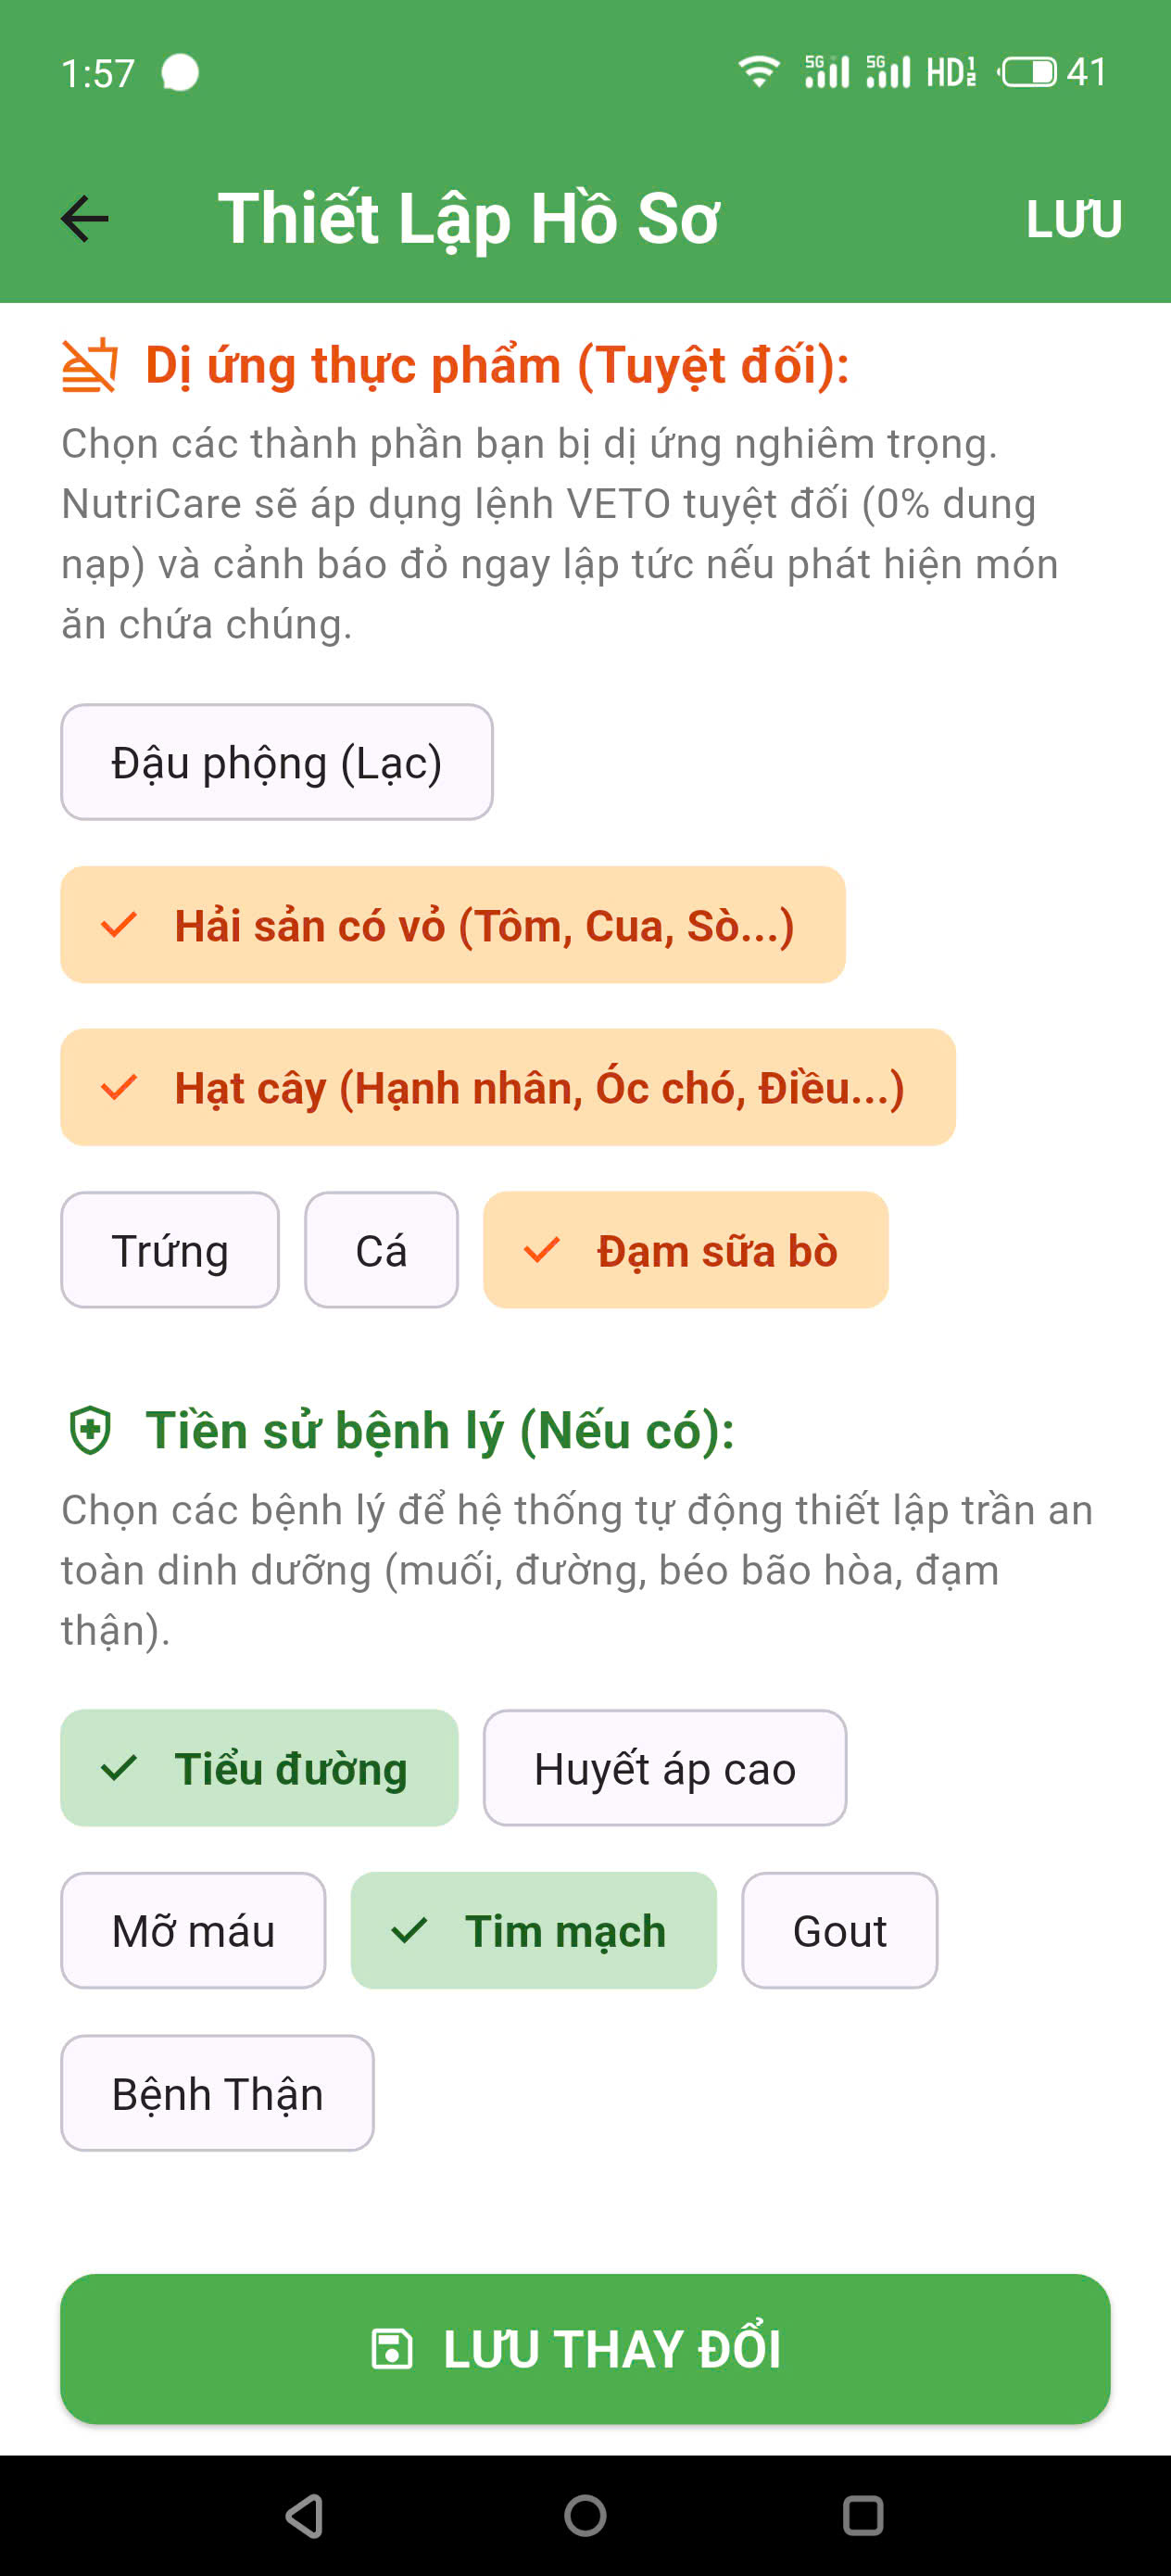
\includegraphics[width=0.88\textwidth,height=0.46\textheight,keepaspectratio]{hinh3_8b_thiet_lap_duoi.jpg}}
        \par\vspace{4pt}{\small (b) Phần dưới: chọn dị ứng và tiền sử bệnh lý}
    \end{minipage}}
    \caption{Giao diện Màn hình Thiết lập Hồ sơ Sức khỏe}
    \label{fig:ui_edit_profile}
\end{figure}

\begin{figure}[htbp]
    \centering
    {\setlength{\fboxsep}{0pt}\setlength{\fboxrule}{0.4pt}%
    \begin{minipage}[b]{0.46\textwidth}
        \centering
        \fcolorbox{black!15}{white}{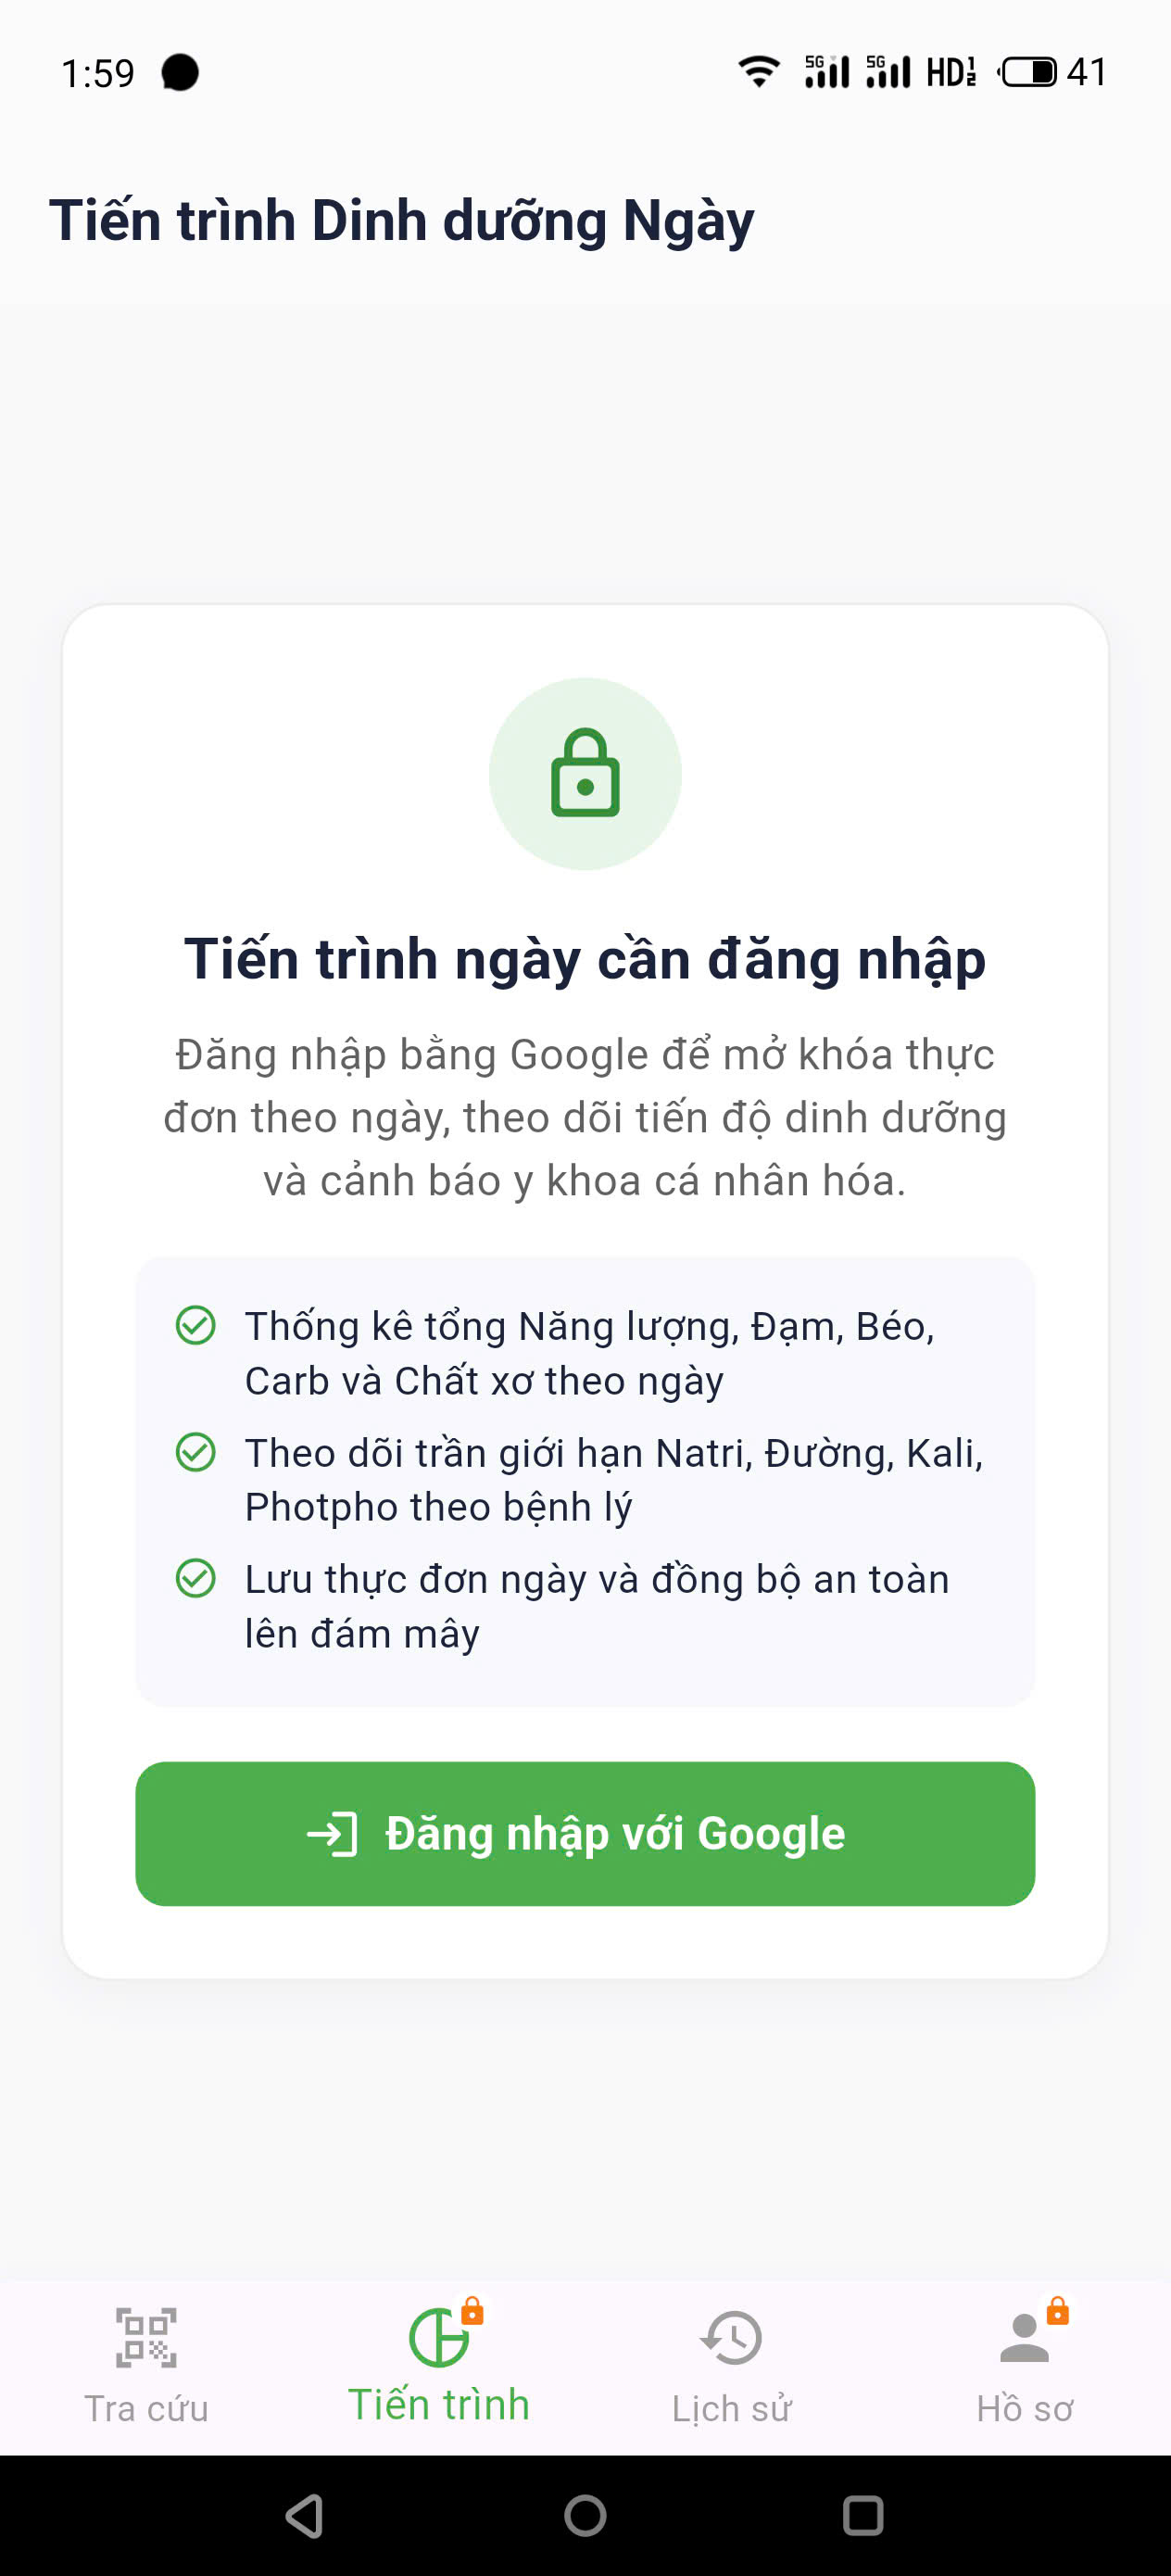
\includegraphics[width=0.88\textwidth,height=0.46\textheight,keepaspectratio]{hinh3_9a_khach_tien_trinh.jpg}}
        \par\vspace{4pt}{\small (a) Khóa tính năng trên Tab Tiến trình}
    \end{minipage}
    \hfill
    \begin{minipage}[b]{0.46\textwidth}
        \centering
        \fcolorbox{black!15}{white}{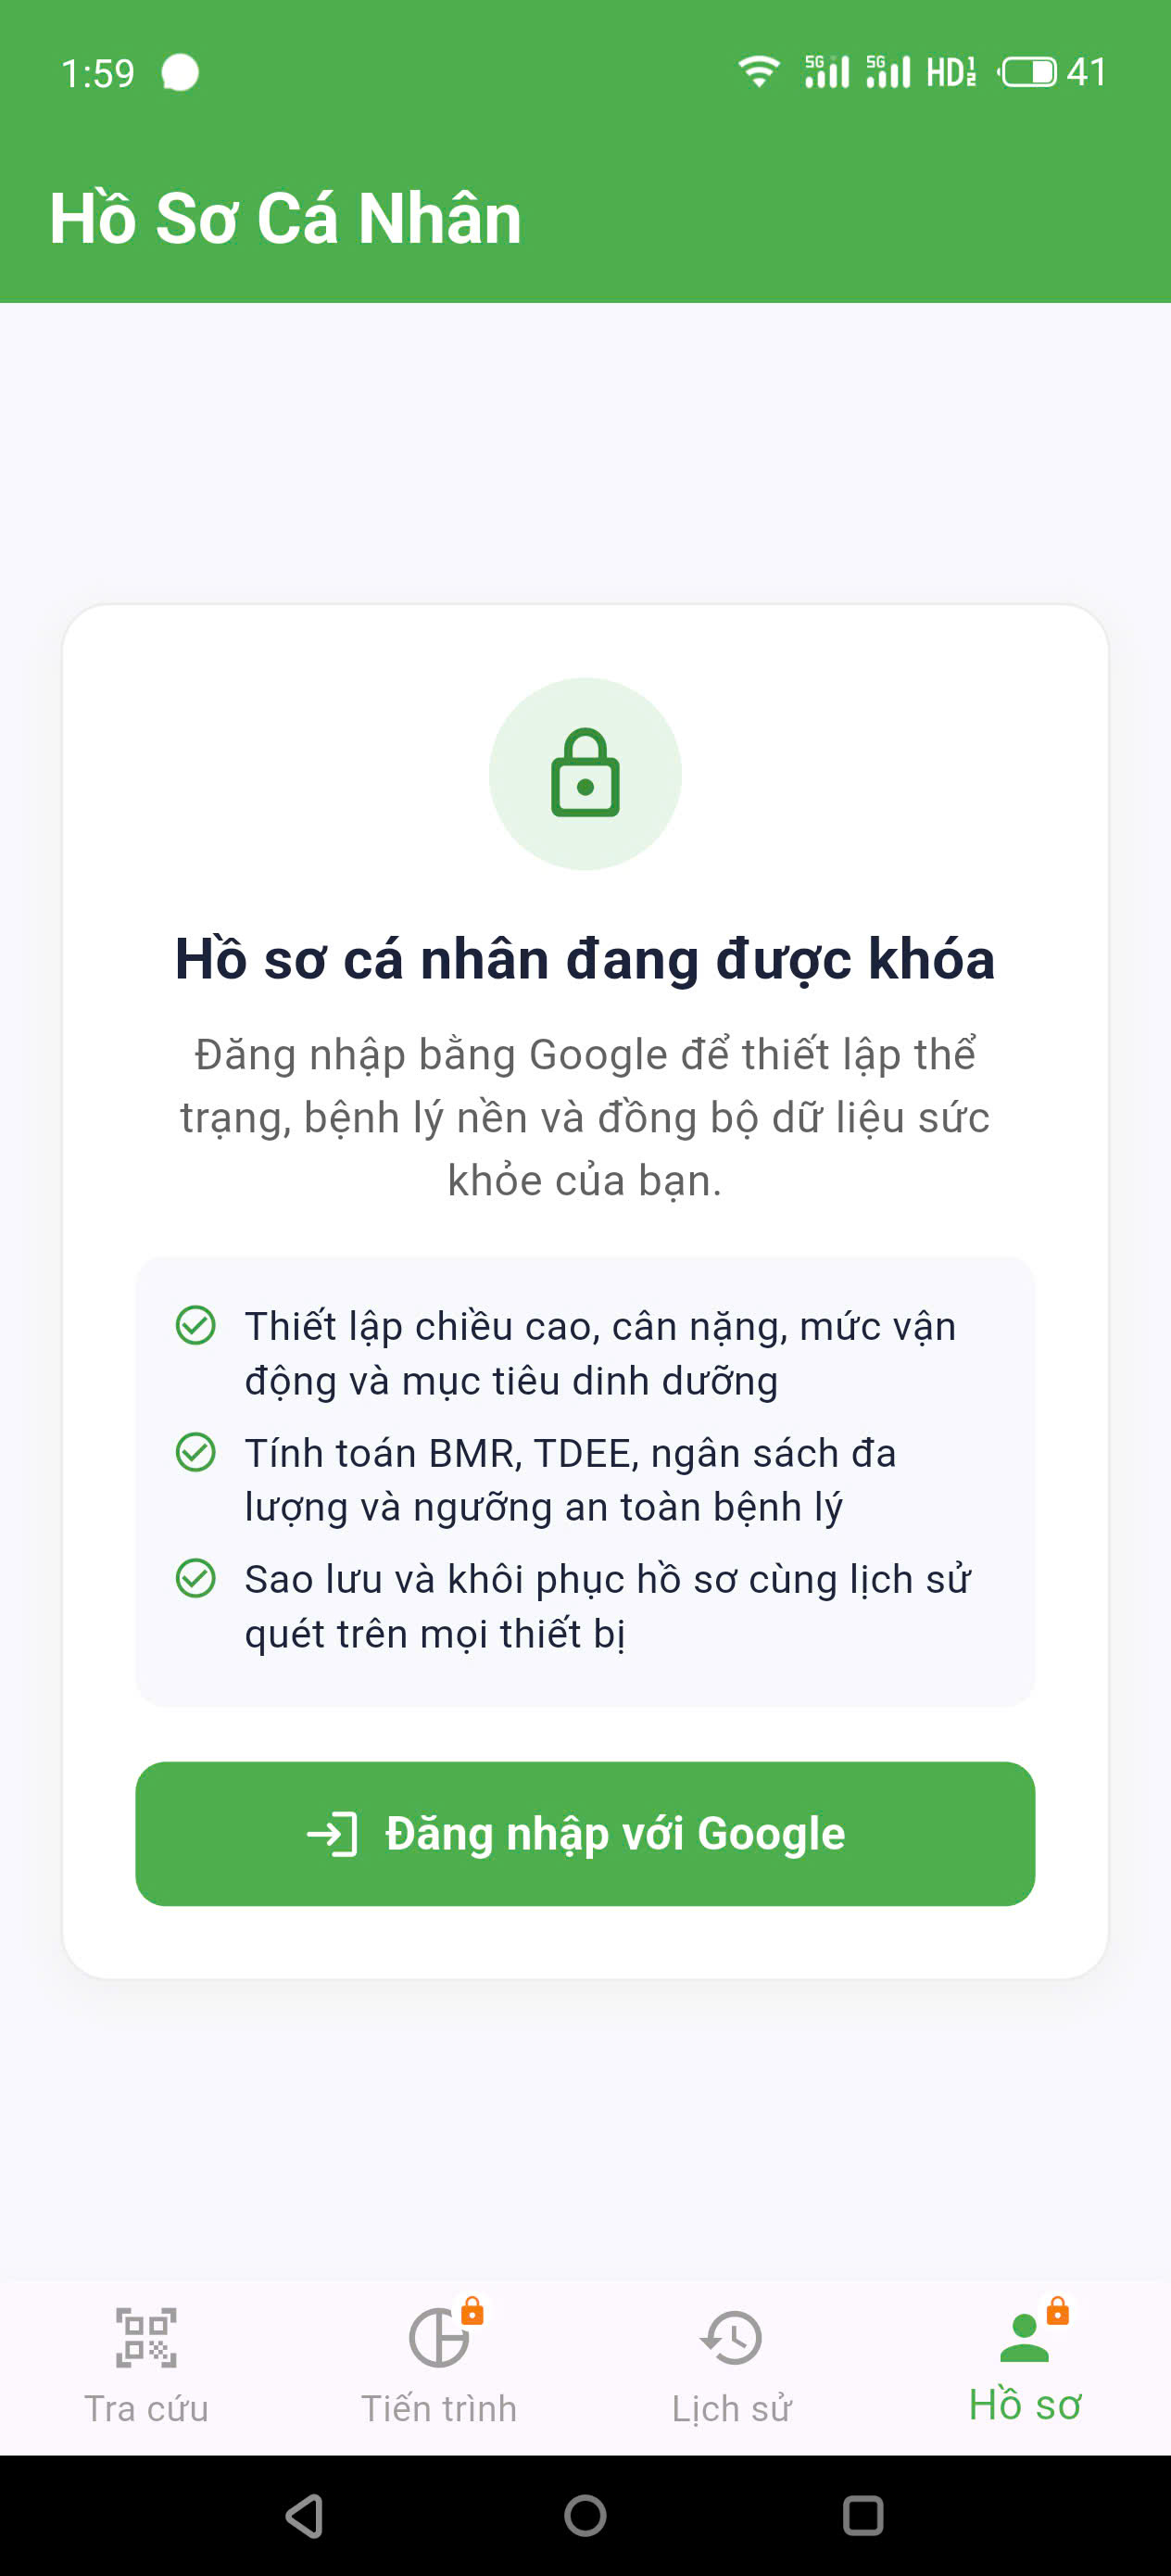
\includegraphics[width=0.88\textwidth,height=0.46\textheight,keepaspectratio]{hinh3_9b_khach_ho_so.jpg}}
        \par\vspace{4pt}{\small (b) Khóa tính năng trên Tab Hồ sơ}
    \end{minipage}}
    \caption{Trạng thái khóa chức năng và nút đăng nhập tại chỗ ở chế độ Khách}
    \label{fig:ui_guest_locked}
\end{figure}
